% ============================================================================
%  A Data-Analysis Agent, Built From Scratch
%  Part 1: a review of two benchmark papers.  Part 2: the design, and how I'd
%  know it works.
%
%  Traditional academic Beamer (Madrid + Palatino).  Compile with:
%      latexmk -pdf presentation.tex
%
%  PROVENANCE.  Every claim about the PAPERS was verified against the PDFs in
%  papers/ by a full re-read (see docs/PART1_REVIEW.md).  Every quantitative
%  claim about MY system comes from `uv run python -m evals.report`
%  (evals/results.jsonl, 4,480 runs) -- not from prose.  Where DESIGN.md and
%  the script disagreed, the script won; the exceptions are noted on the
%  colophon frame.
% ============================================================================
\documentclass[9pt,aspectratio=169]{beamer}

% ---- a traditional academic look -------------------------------------------
\usetheme{Madrid}
\usefonttheme{serif}
\usepackage[T1]{fontenc}
\usepackage{mathpazo}                    % Palatino: the academic serif
\usepackage[scaled=0.78]{beramono}       % a mono that sits well next to Palatino
\usepackage{microtype}

\usepackage{booktabs}
\usepackage{array}
\usepackage{amsmath,amssymb}
\usepackage{xcolor}
\usepackage{tikz}
\usepackage{listings}
\usetikzlibrary{arrows.meta, positioning, shapes.geometric, fit, backgrounds}

% ---- restraint: no navigation clutter, tight lists -------------------------
\setbeamertemplate{navigation symbols}{}
\setbeamertemplate{caption}[numbered]
\setbeamersize{text margin left=5mm, text margin right=5mm}
\setlength{\parskip}{0pt}
\usepackage{etoolbox}
\AtBeginEnvironment{itemize}{\setlength{\itemsep}{2.5pt}\setlength{\topsep}{2pt}}
\AtBeginEnvironment{enumerate}{\setlength{\itemsep}{2.5pt}\setlength{\topsep}{2pt}}
\AtBeginEnvironment{tabular}{\setlength{\extrarowheight}{1.5pt}}
\AtBeginEnvironment{block}{\small}
\AtBeginEnvironment{alertblock}{\small}
\AtBeginEnvironment{exampleblock}{\small}
\setbeamertemplate{itemize/enumerate body begin}{\small}
\setbeamertemplate{itemize/enumerate subbody begin}{\footnotesize}
\setbeamertemplate{blocks}[rounded][shadow=false]
\setbeamertemplate{title page}[default][colsep=-4bp,rounded=true,shadow=false]

% ---- a restrained academic palette -----------------------------------------
\definecolor{unired}{HTML}{9B2226}
\definecolor{unigreen}{HTML}{1B5E3F}
\definecolor{uniamber}{HTML}{8A5A00}
\definecolor{unigrey}{HTML}{5A5A5A}
\definecolor{unipale}{HTML}{EEF1F6}
\setbeamercolor{alerted text}{fg=unired}

\newcommand{\gd}[1]{\textcolor{unigreen}{\textbf{#1}}}
\newcommand{\rd}[1]{\textcolor{unired}{\textbf{#1}}}
\newcommand{\wn}[1]{\textcolor{uniamber}{\textbf{#1}}}
\newcommand{\sm}[1]{{\color{unigrey}\small #1}}
\newcommand{\code}[1]{\texttt{\small #1}}
\newcommand{\yes}{\textcolor{unigreen}{$\checkmark$}}
\newcommand{\no}{\textcolor{unired}{$\times$}}

% a quiet "why this slide exists" strip under the frametitle
\newcommand{\why}[1]{{\color{unigrey}\footnotesize\itshape #1\par\vspace{4pt}}}
% A source tag, because every number in this deck has one. It must open its own paragraph --
% otherwise, following a tabular, it wraps up alongside the last row instead of sitting under it.
\newcommand{\src}[1]{\par\vspace{2pt}{\color{unigrey}\scriptsize #1}\par}

\lstdefinestyle{py}{
  language=Python,
  basicstyle=\ttfamily\footnotesize,
  commentstyle=\color{unigrey}\itshape,
  keywordstyle=\color{structure}\bfseries,
  stringstyle=\color{unigreen},
  showstringspaces=false, columns=fullflexible, keepspaces=true,
  aboveskip=3pt, belowskip=3pt,
}
\lstset{style=py}

\title[A Data-Analysis Agent]{A Data-Analysis Agent, Built From Scratch}
\subtitle{Part 1: two benchmark papers on autonomous scientific analysis\\
          Part 2: a design built against what they found}
\author[M. Tabares Pardo]{Musel Tabares Pardo}
\institute[]{}
\date[July 2026]{July 2026}

\begin{document}

\begin{frame}[plain]
\maketitle
\end{frame}

% ===========================================================================
\begin{frame}{What this talk is}
\begin{block}{Two papers, one system}
Both supplied papers evaluate \textbf{the same thing}: a single LLM agent, alone in a container,
writing and running code against messy scientific data, returning one structured answer.
\end{block}
\medskip
That is \emph{exactly} the system Part 2 asks me to build. So the papers are not background
reading --- they are \textbf{failure data for the thing I am about to construct}.
\medskip
\begin{columns}[T]
\begin{column}{0.48\textwidth}
\textbf{Part 1 --- the papers}
\begin{itemize}
  \item What are they addressing, and why
  \item What they measured, and what they found
  \item \textbf{How these agents actually fail} --- the intuitions
  \item What convinces me; what does not
  \item The limitation neither paper states
\end{itemize}
\end{column}
\begin{column}{0.48\textwidth}
\textbf{Part 2 --- the design}
\begin{itemize}
  \item The base: an LLM and a loop
  \item \textbf{The gates I add on top, and why each one}
  \item How each gate answers a failure in Part 1
  \item How I would know whether it worked
  \item A live dashboard
\end{itemize}
\end{column}
\end{columns}
\end{frame}

% The outline is shown in two columns, one per Part. NOTE: \tableofcontents is scoped to the
% CURRENT part by default, so the part=N argument is load-bearing -- without it the second
% column silently renders empty.
\newcommand{\outlineframe}{%
\begin{frame}{Outline}
\setbeamertemplate{section in toc}[sections numbered]
{\small
\begin{columns}[T]
\begin{column}{0.49\textwidth}
  {\usebeamercolor[fg]{structure}\textbf{Part I --- The papers}}\par\smallskip
  \tableofcontents[part=1, currentsection, hideallsubsections]
\end{column}
\begin{column}{0.49\textwidth}
  {\usebeamercolor[fg]{structure}\textbf{Part II --- The design}}\par\smallskip
  \tableofcontents[part=2, currentsection, hideallsubsections]
\end{column}
\end{columns}}
\end{frame}}

\outlineframe
\AtBeginSection[]{\outlineframe}

% ###########################################################################
\part{The papers}
\begin{frame}[plain]
\centering\vfill
{\usebeamercolor[fg]{structure}\Huge\textbf{Part I}}\\[10pt]
{\Large The papers}\\[16pt]
{\color{unigrey}\normalsize Two benchmarks for autonomous scientific analysis ---\\
what they found, and where I think they are wrong}
\vfill
\end{frame}

\section{Context: what the two papers are addressing}
% ###########################################################################

\begin{frame}{The system under evaluation --- concretely}
\why{Before any result, be precise about what is actually being tested. Neither paper is about chatbots.}

\begin{block}{An ``autonomous scientific analysis agent''}
\begin{enumerate}
  \item An LLM is dropped into a \textbf{sandboxed container} with Python, \code{pandas}/\code{scipy}/\code{statsmodels}, and scientific data files.
  \item It is given a scientific question \textbf{stated at a high level} --- and \emph{deliberately not} told how to answer it.
  \item It must \textbf{decide the method itself}: which rows to keep, which estimator, which filters, when the evidence suffices.
  \item It \textbf{writes and executes its own code}, in a loop, reading its own output.
  \item It returns \textbf{one machine-checkable answer} --- a JSON object, or a file.
\end{enumerate}
\end{block}
\pause
\begin{itemize}
  \item No human in the loop. No hints. \textbf{Grading is all-or-nothing} in both papers.
  \item \textbf{GeneBench-Pro} (Li \& Ho, OpenAI --- bioRxiv preprint, 30 June 2026): 129 problems, genomics and translational biomedicine.
  \item \textbf{DrugDiscoveryBench} (Aky\"urek, Tu et al., Scale AI \& Phylo, 2026): 82 tasks, early-stage drug discovery.
\end{itemize}
\sm{Both are preprints --- GBP explicitly ``not certified by peer review''; DDB prints no venue at all.}
\end{frame}

\begin{frame}{Why anyone is asking this question}
\why{The motivation is economic, and both papers reach for the same argument.}

\begin{columns}[T]
\begin{column}{0.5\textwidth}
\textbf{The bottleneck moved.}
\medskip

Sequencing got cheap. Generating data is no longer the hard part.
\medskip

\begin{quote}\footnotesize\itshape
``as sequencing has scaled, downstream computation and analysis, rather than data generation, have
become the central scientific bottleneck.''
\end{quote}
\src{GeneBench-Pro, p.\,2}
\end{column}
\begin{column}{0.5\textwidth}
\textbf{And the stakes are real.}
\medskip

Drug targets with human genetic evidence are
\medskip

\begin{quote}\footnotesize\itshape
``roughly 2.6 times more likely to succeed in the clinic''
\end{quote}
\src{DrugDiscoveryBench, p.\,2 (Minikel et al., \emph{Nature} 2024)}
\medskip

\sm{GBP costs it out: one of their problems takes a human expert \textbf{10--40 hours} at \$100--200/hr
--- ``on the order of a few thousand dollars'' each (p.\,14, and they flag it as illustrative).}
\end{column}
\end{columns}
\pause
\medskip
\begin{alertblock}{So the question is worth a benchmark}
If an agent could reliably do this analysis, it would compress the slowest, most expensive step in
data-rich biology. \textbf{Can it?}
\end{alertblock}
\end{frame}

\begin{frame}{What existing benchmarks measured --- and missed}
\why{GBP's Figure 1 is the whole argument for why these papers exist.}

\begin{columns}[T]
\begin{column}{0.47\textwidth}
\begin{block}{What prior benchmarks test}
\centering\footnotesize
curated dataset\\ $\downarrow$ \\ a well-defined, routine analysis \\ $\downarrow$ \\ a result
\end{block}
\sm{The method is \emph{given}. The agent executes it. This measures \textbf{execution}.}
\end{column}
\begin{column}{0.53\textwidth}
\begin{block}{What real scientific analysis is}
\centering\footnotesize
data of \textbf{unknown quality}\\ $\downarrow$ \\ EDA / QC / preprocessing \\ $\downarrow$ \\
modelling \& inference $\rightleftarrows$ \textbf{diagnostics} \\ $\downarrow$ \\ a decision-relevant conclusion
\end{block}
\sm{The method must be \textbf{chosen}, and re-chosen as diagnostics come back. This measures \textbf{judgement}.}
\end{column}
\end{columns}
\pause
\medskip
\begin{quote}\small\itshape
``Its core challenges stem not from the execution of analytical workflows, but from the importance
of scientific intuition or \textbf{`research taste'}: chains of judgment calls about what question the
data can support, what data to include, which estimand or model is appropriate, whether diagnostics
invalidate initial hypotheses, and when the evidence is strong enough to support a conclusion.''
\end{quote}
\src{GeneBench-Pro, p.\,2 --- verbatim}
\end{frame}

\begin{frame}{The one idea that makes the benchmark diagnostic}
\why{GBP's central construct. It is the reason the benchmark is hard \emph{in an interesting way}.}

\begin{block}{The \emph{decision point}}
\begin{quote}\itshape
``substantive inferential forks where a plausible wrong choice leads to a qualitatively different
downstream answer''
\end{quote}
\src{GeneBench-Pro, p.\,7 --- verbatim. Range \textbf{3--13 per problem}, median \textbf{6}.}
\end{block}
\pause
\medskip
This is the difference between a benchmark that is \textbf{hard} and one that is \textbf{diagnostic}:
\medskip
\begin{itemize}
  \item A problem can be hard because the arithmetic is fiddly. That tells you nothing.
  \item A GBP problem is hard because there are \textbf{six places to take a defensible-looking wrong turn} --- and the wrong turn lands you somewhere \emph{measurably} else.
  \item And the errors \textbf{cascade}: \sm{``an incorrect choice at any stage propagates into downstream errors and ultimately failure to recover the final correct target'' (p.\,5)}.
\end{itemize}
\pause
\medskip
\begin{alertblock}{This is the idea I stole outright for my own evaluation}
Plant the fork. Know where the wrong path lands. Then you can say not just \emph{that} the agent was
wrong, but \textbf{which wrong}.
\end{alertblock}
\end{frame}

% ###########################################################################
\section{The two benchmarks, and what they found}
% ###########################################################################

\begin{frame}{GeneBench-Pro --- the setup}
\begin{columns}[T]
\begin{column}{0.54\textwidth}
\begin{itemize}
  \item \textbf{129 problems}, 10 primary domains, 21 subdomains.
  \item \textbf{Fully simulated} data --- so the causal structure is known and nothing can be memorised.
  \item Docker, \textbf{no internet}. A deliberately minimal prompt.
  \item \textbf{Binary, programmatic grading.} Pre-specified target fields, absolute numeric tolerances. \textbf{No LLM judge anywhere.}
  \item \textbf{10 attempts} per model--problem \sm{(5 for the GPT Pro (Extended) and Claude Opus rows --- 11 of 60)}.
  \item 60 model configurations; 95\% CIs by hierarchical bootstrap, 20,000 resamples.
  \item 82 of 129 problems reviewed by \textbf{11 external domain experts}.
\end{itemize}
\end{column}
\begin{column}{0.46\textwidth}
\begin{block}{The best design choice in either paper}
They simulate the data --- but they \textbf{do not grade against the simulation parameter}. They grade
against \emph{the estimate a correct analyst could actually recover from the staged files}.
\medskip

\sm{Otherwise sampling noise in the DGP marks a correct analysis wrong. Table 1 (p.\,6) names that
exact failure mode. This is subtle, and right.}
\end{block}
\end{column}
\end{columns}
\end{frame}

\begin{frame}{GeneBench-Pro --- the results are brutal}
\centering
\small
\begin{tabular}{@{}lrl@{}}
\toprule
\textbf{Configuration} & \textbf{Pass rate} & \textbf{95\% CI} \\
\midrule
GPT-5.6 Sol Pro (Extended) --- \emph{best in paper} & \textbf{31.5\%} & [24.3, 38.9] \\
GPT-5.6 Sol (max) --- \emph{best mainline}          & \textbf{28.7\%} & [22.5, 35.1] \\
GPT-5.6 Terra (max)                                  & 23.3\% & [17.8, 29.2] \\
GPT-5.6 Luna (max)                                   & 16.5\% & [11.6, 21.7] \\
Claude Opus 4.8 (max) --- \emph{strongest non-GPT}   & 16.0\% & [11.0, 21.2] \\
GPT-5.5 (xhigh)                                      & 12.0\% & \\
\midrule
\multicolumn{3}{@{}l@{}}{\sm{Non-GPT range across all rows: \textbf{0.6\%} (MiniMax M2.7) to 16.0\% (Claude Opus 4.8)}}\\
\bottomrule
\end{tabular}
\src{Supplementary Table 1, p.\,21}

\pause
\medskip
\begin{columns}[T]
\begin{column}{0.5\textwidth}
\begin{alertblock}{The number that should stop you}
The best mainline model scores \rd{zero across all ten attempts on 45.7\% of problems.}
\medskip
\sm{Nearly half the benchmark is never solved once, by the best model, in ten tries.}
\end{alertblock}
\end{column}
\begin{column}{0.5\textwidth}
\begin{block}{Reasoning effort buys a lot --- then saturates}
GPT-5.6 Sol, \emph{none} $\to$ \emph{max}:
\smallskip

\centering
3.7\% $\to$ 14.4 $\to$ 22.5 $\to$ 24.4 $\to$ 26.8 $\to$ \textbf{28.7\%}
\smallskip

\raggedright\sm{An 8$\times$ gain from inference compute alone --- but high$\to$max buys only 1.9 points.}
\end{block}
\end{column}
\end{columns}
\end{frame}

\begin{frame}{DrugDiscoveryBench --- the setup}
\begin{columns}[T]
\begin{column}{0.54\textwidth}
\begin{itemize}
  \item \textbf{82 expert-authored tasks}, target identification $\to$ patent mining $\to$ structure--activity analysis.
  \item Grounded in \textbf{real artifacts}: granted patents, PDB structures, papers, database records.
  \item Environment: an adaptation of Stanford's \textbf{BIOMNI} --- 226 functions across 22 domains, a 76-file data lake. \textbf{Internet on.}
  \item Graded by an \textbf{LLM judge} (GPT-5.4) against weighted expert rubrics. \textbf{Pass = 100\% of outcome criteria.}
  \item \textbf{12 models $\times$ 6 harnesses}, 29 settings, \textbf{3 trials} each.
  \item Six-gate authoring pipeline, with a \emph{drop rule} for tasks that cannot be made robust.
\end{itemize}
\end{column}
\begin{column}{0.46\textwidth}
\begin{block}{Best agent: \textbf{51.6\%}}
\centering\small
GPT-5.5 + mini-SWE-agent (xhigh)
\end{block}
\begin{block}{Two findings worth the price of admission}
\footnotesize
\textbf{1. Test-time compute scales} --- within a family.\\
GPT-5.5 (Codex): 27.6 $\to$ 39.8 $\to$ \textbf{43.9\%}
\medskip

\textbf{2. The harness matters as much as the model.}\\
GPT-5.5 swings \textbf{40.6 $\to$ 51.6\%} across harnesses --- an 11-point spread. The gap between
the \#1 and \#2 \emph{models} is \textbf{1.6 points}.
\end{block}
\end{column}
\end{columns}
\end{frame}

\begin{frame}{The two, side by side --- and a warning}
\centering\footnotesize
\begin{tabular}{@{}p{0.16\textwidth}p{0.38\textwidth}p{0.38\textwidth}@{}}
\toprule
 & \textbf{GeneBench-Pro} & \textbf{DrugDiscoveryBench} \\
\midrule
\textbf{Tasks}       & 129, \textbf{fully simulated} & 82, \textbf{expert-authored on real artifacts} \\
\textbf{Domain}      & Genomics, translational biomedicine & Early-stage drug discovery \\
\textbf{Ground truth}& Computable by construction & Written by pharmaceutical scientists \\
\textbf{Grader}      & \gd{Deterministic Python. No LLM.} & \rd{LLM judge (GPT-5.4) + rubric} \\
\textbf{Internet}    & \gd{Off} & \rd{On} (and it leaked --- see later) \\
\textbf{Runs/cell}   & 10 \sm{(5 for some rows)} & 3 \\
\textbf{Harness}     & Fixed --- not a variable & \gd{A first-class variable (6 of them)} \\
\textbf{Failure data}& Qualitative only, \rd{no frequencies} & \gd{A 5-way taxonomy with frequencies} \\
\midrule
\textbf{Headline}    & \textbf{28.7\%} (mainline) / 31.5\% (Pro) & \textbf{51.6\%} \\
\bottomrule
\end{tabular}

\pause
\medskip
\begin{alertblock}{Do not compare 28.7\% with 51.6\%}
They are not on the same scale. DDB's tasks were \textbf{pre-screened to be solvable} with the
expert's playbook (a solvability gate in construction). And GBP's own independently-held-out subset
drops the same model from \textbf{28.7\% to 16.3\%}. The two numbers measure different things on
different sets.
\end{alertblock}
\end{frame}

% ###########################################################################
\section{How these agents actually fail}
% ###########################################################################

\begin{frame}{The single most useful table in either paper}
\why{DDB classified 226 failing runs into a root-cause taxonomy. This is what a builder needs.}

\centering\small
\begin{tabular}{@{}lrp{0.50\textwidth}@{}}
\toprule
\textbf{Failure mode} & \textbf{Share} & \textbf{Their definition} \\
\midrule
\rd{Domain reasoning} & \rd{54.0\%} & ``applies an incorrect scientific premise or misinterprets the data it has, \textbf{even though its inputs and tools are correct}'' \\
Derivation error      & 18.6\% & right approach, wrong calculation \\
Retrieval             & 16.4\% & wrong source, or never reads a provided file \\
Constraint            & 7.5\%  & violates an explicit instruction in the prompt \\
Final-answer slip     & 3.5\%  & every step right, reports the answer wrongly \\
\bottomrule
\end{tabular}
\src{DrugDiscoveryBench, Table 3, p.\,11 --- $n=226$ failing runs}

\pause
\medskip
\begin{alertblock}{Read the top row again}
\textbf{Over half of all failures are not coding failures.} The tools worked. The Python ran. The
data was right there.
\medskip

\sm{(I will come back and attack this table's methodology. But qualitatively it is the most useful
artifact in either paper, and I reuse its five categories verbatim so my own failure profile is
comparable to the literature.)}
\end{alertblock}
\end{frame}

\begin{frame}{Failure 1 --- it notices, and then does nothing about it}
\why{GBP's central diagnosis. If you remember one thing from Part 1, remember this.}

\begin{quote}\itshape
``models often complete substantial portions of the workflow but exhibit a consistent gap between
\textbf{noticing} and \textbf{acting} by identifying local diagnostic signals but failing to
propagate the implications to the corresponding analysis decision. As a result, models often select
wrong estimators or persist on initially plausible but incorrect analysis paths.''
\end{quote}
\src{GeneBench-Pro, abstract, p.\,1 --- verbatim}
\pause
\medskip
\begin{quote}\itshape
``the agent \textbf{notices} the relevant local diagnostic clue but \textbf{treats it as a local data
cleaning issue rather than as evidence that should change the downstream statistical method and QC
pipeline}.''
\end{quote}
\src{GeneBench-Pro, p.\,13 --- verbatim}
\pause
\medskip
\begin{block}{The intuition, in one sentence}
The model \emph{sees} the problem. It runs \code{df.describe()}. It observes the sentinel values. It may
even print a comment about them. \textbf{Then it cleans the column and proceeds with the analysis it had
already decided on.}
\medskip

\centering\textbf{The observation never reaches the decision.}
\end{block}
\end{frame}

\begin{frame}{Failure 2 --- the question quietly degrades}
\why{The one I find most alarming, because nothing crashes and the arithmetic is correct.}

\begin{block}{DDB, the melanoma task (c4222f)}
\textbf{Asked:} which gene is the melanoma marker?\\
\textbf{What happens:} somewhere mid-trajectory the qualifier \emph{``melanoma''} silently falls out.
The ranking becomes a \emph{gene-wide} variant count. \textbf{PTEN} wins on sheer volume --- driven by
non-melanoma syndromes. \sm{(Truth: CDKN2A.)}
\end{block}
\pause
\begin{block}{GBP, the DRX1 problem}
The estimand is the average carrier probability over \textbf{the entire roster}. The agent standardises
over \textbf{tested partners only} --- a different denominator, a plausible answer, and the wrong one.
\end{block}
\pause
\medskip
\begin{alertblock}{The pattern}
\textbf{A constraint or a population silently drops out of the question partway through a long
trajectory}, and every step after that is a correct analysis \emph{of the wrong question}.
\medskip

GBP names the end state exactly: \emph{``A statistically valid final model is applied to the wrong data
or population, on the wrong scale, or on the wrong conceptual level.''} \src{(p.\,6)}
\end{alertblock}
\end{frame}

\begin{frame}{Failure 3 --- the right method, applied to the wrong object}
\begin{block}{DDB, the net-charge task (e3c637)}
The chemistry is \textbf{correct}. The method is \textbf{correct}. It is executed on the neutral
\textbf{reference} molecule instead of the \textbf{bound ligand}.
\medskip

Answer: \textbf{0}. Truth: \textbf{$-$1}.
\end{block}
\pause
\medskip
\begin{alertblock}{And here is the part that should worry anyone building a self-checking agent}
The agent ran \textbf{three internal consistency checks}. All three \textbf{agreed}. All three were run
\textbf{on the wrong molecule}.
\medskip

\centering\textbf{Internal consistency is not validity.}
\end{alertblock}
\pause
\medskip
\sm{The design consequence, which I take seriously in Part 2: \textbf{do not trust the agent's own
reasoning trace, or its own agreement with itself, as a validity signal.} A verifier that reads the
agent's narrative will agree with the agent's narrative. Verification has to come from
\emph{outside} the trajectory --- or from something that cannot be argued with at all.}
\end{frame}

\begin{frame}{Failure 4 --- its own code printed the right number}
\why{My favourite failure in either paper, because it is so cheap to prevent.}

\begin{quote}\large\itshape
``its own code printed the correct group-level count of 1, but the final tally used the atom-level
count of 2\ldots{} It reported 8 interactions instead of 7.''
\end{quote}
\src{DrugDiscoveryBench, task bf9c6d, p.\,27 --- verbatim}

\pause
\medskip
\begin{itemize}
  \item The analysis was \textbf{right}.
  \item The code was \textbf{right}.
  \item The output on screen was \textbf{right}.
  \item \rd{The number in the answer was not the number in the output.}
\end{itemize}
\pause
\medskip
\begin{exampleblock}{This is a \emph{15-line regex} away from being impossible}
An LLM reviewer \emph{might} catch this. A deterministic check --- \emph{``every number you report must
appear verbatim in the stdout of code that actually ran''} --- catches it \textbf{every time, for free}.
\medskip

This becomes Gate 3 in Part 2, and it is the cheapest mechanism in my entire design.
\end{exampleblock}
\end{frame}

\begin{frame}{Failure 5 --- nobody checks the answer at the end}
\begin{quote}\itshape
``\textbf{The last chance to catch the slip is at the final answer}: a human who had misread the task
the same way would look at the result, recognize it as a meaningless response to the user's actual
goal, and backtrack. \textbf{None of the failing models caught this.}''
\end{quote}
\src{DrugDiscoveryBench, p.\,13 --- verbatim}

\pause
\medskip
\begin{block}{What that looks like in practice}
Claude Opus answers \textbf{BRCA2} --- a \emph{breast}-cancer gene --- to a \textbf{melanoma} question.
\medskip

Any domain expert glancing at that output would stop dead. \textbf{The agent submits it.}
\end{block}
\pause
\medskip
\begin{alertblock}{The summary sentence of the whole failure story}
\begin{quote}\itshape
``the agents knew which database to query and how to compute the property the task asked for at a high
level. But somewhere along the execution they \textbf{drop a constraint, commit too early, fail to
backtrack} or fail with respect to scientific common sense.''
\end{quote}
\src{DrugDiscoveryBench, p.\,12 --- verbatim}
\end{alertblock}
\end{frame}

\begin{frame}{The takeaway --- and it is not ``the models are bad''}
\begin{block}{Two labs. Two domains. Two grading philosophies. \textbf{One diagnosis.}}
\begin{quote}\itshape
``their failures are seldom about missing biological facts, more often they involve \textbf{losing the
scientific thread of the task}\ldots{} A central missing capability is sound scientific reasoning and
judgment, including \textbf{keeping the original scientific objective active while executing many local
tool calls and intermediate decisions}.''
\end{quote}
\src{DrugDiscoveryBench, p.\,16 --- verbatim}
\end{block}
\pause
\medskip
And the result that says where the headroom is:
\medskip
\begin{itemize}
  \item \textbf{76 of 82} tasks are solved without hints by \emph{at least one} agent in \emph{at least one} trial.
  \item Hand the 6 stragglers \textbf{the expert's step-by-step playbook}, and \textbf{80 of 82} pass \sm{(``and near-pass 1'')}.
\end{itemize}
\pause
\medskip
\begin{alertblock}{The conclusion both papers earn}
\begin{quote}\itshape
``\textbf{execution is within reach for today's agents should they be given the expert workflow.}''
\src{(DDB, p.\,14)}
\end{quote}
\centering\medskip
The bottleneck is not code generation, not knowledge, and not context length. It is
\textbf{procedure} --- and \textbf{procedure is something an engineer can build.}
\end{alertblock}
\end{frame}

% ###########################################################################
\section{What is convincing --- and what is not}
% ###########################################################################

\begin{frame}{What is convincing --- GeneBench-Pro's benchmark design}
\why{This is the best thing in either paper, and I copied it wholesale.}

\begin{enumerate}
  \item \textbf{Simulate, so you can \emph{compute} the truth.} Real data gives ground truth you can
        \emph{assume}. Simulation gives ground truth you can \emph{calculate} --- and it is the only way
        to \emph{plant} a decision point and be certain the naive path lands somewhere else.
  \pause
  \item \textbf{Grade the recoverable estimate, not the generating parameter.} Subtle and correct:
        otherwise sampling noise in your own simulator marks a \emph{correct} analysis wrong.
  \pause
  \item \textbf{Ablation-verify the separation.} For every trap, assert that the plausible-but-wrong
        answer lies \emph{far outside} the tolerance band. Otherwise a lazy analysis lands inside the
        band and is graded correct --- and \textbf{the benchmark measures nothing.}
  \pause
  \item \textbf{Be robust to defensible analyst variation.} \emph{``nearby reasonable thresholds lead to
        the same graded outcome''} (p.\,6). Otherwise you are measuring luck at the cutoff lottery
        rather than recognition of the problem.
  \pause
  \item \textbf{Binary, all-or-nothing grading}, and they defend it better than I could:
        \begin{quote}\footnotesize\itshape
        ``an agent that executes several intermediate steps correctly but returns the wrong
        decision-relevant answer has not successfully automated the analysis.'' \src{(p.\,14)}
        \end{quote}
        Partial credit measures effort. Binary measures usefulness.
\end{enumerate}
\end{frame}

\begin{frame}{What is convincing --- the unglamorous, expensive, right things}
\begin{block}{GBP: there is \emph{no LLM judge}. At all.}
Grading is deterministic Python against pre-specified fields and tolerances. So the entire
``was the judge validated?'' question --- which sinks a lot of agent papers --- \textbf{simply does not
arise} for GBP's numbers.
\end{block}
\pause
\begin{block}{GBP: external review caught errors in \emph{the authors' own ground truth}, and they published them}
Table 2 (p.\,9) prints the reviewers' catches \emph{against the authors} --- including a reference
implementation that was \emph{``not implementing actual LDSC''}, and a simulator with a
\emph{``faulty formula''}. \textbf{Admitting in print that your grader was scoring correct answers as
wrong is a strong trust signal}, and rare.
\end{block}
\pause
\begin{block}{DDB: expert authorship, and the harness as a variable}
82 tasks written by pharmaceutical scientists against real patents is \textbf{the part you cannot
fake or generate}. And treating the \textbf{scaffold} as a first-class experimental variable is
something most agent papers do not do --- \emph{and it turns out to matter more than the model}.
\end{block}
\pause
\smallskip
\centering\textbf{And both papers publish their failure modes, not just their scores.}\\
\sm{That is rarer than it should be, and it is the only reason either paper is useful to a builder.}
\end{frame}

\begin{frame}{What is questionable --- GBP's central claim has no numbers behind it}
\why{The notice--act gap is the paper's headline intellectual contribution. Look at what supports it.}

\begin{quote}\large\itshape
``\textbf{Manual review} of model-reported reasoning from \textbf{selected} GPT-5.5 / GPT-5.6 Sol
comparisons \textbf{suggests} a consistent mechanism behind this scaling.''
\end{quote}
\src{GeneBench-Pro, p.\,13 --- verbatim. This is the \emph{entire} evidentiary base, plus three
hand-picked excerpts in Table 3.}

\pause
\medskip
\begin{itemize}
  \item \rd{No $n$.} How many runs were reviewed is never stated.
  \item \rd{No selection rule.} ``Selected'' is doing enormous unexamined work.
  \item \rd{No coding scheme, no blinding, no inter-rater agreement, no rate.} What \emph{fraction} of failures show the pattern? Unanswerable.
\end{itemize}
\pause
\medskip
\begin{alertblock}{And it gets worse: the evidence is the model's \emph{self-report}}
The diagnosis rests on a \textbf{free-text reasoning field}. And:
\begin{itemize}\footnotesize
  \item p.\,7 --- the prompt tells the model that \emph{``analytical reasoning quality is graded alongside numerical correctness''}.
  \item p.\,15 --- \emph{``A free-text reasoning field is also collected for qualitative analysis but is \textbf{not graded}.''}
\end{itemize}
\smallskip
So the model is told its reasoning is graded, it is not, and \textbf{that same text is the sole evidence
for the paper's central claim} --- never once checked against what the code actually did.
\end{alertblock}
\smallskip
\centering\sm{\textbf{The pass rates are solid. The story explaining them is an anecdote with $n$ unstated.}}
\end{frame}

\begin{frame}{What is questionable --- GBP's error bars are not error bars}
\why{This is the criticism I am most confident in, because the paper prints the evidence itself.}

Supplementary Table 2 (p.\,22) reports uncertainty as \emph{``the half-width of a 95\% hierarchical
bootstrap confidence interval''} --- a \textbf{symmetric $\pm$} on a quantity \textbf{bounded below by
zero}. Read literally:

\medskip
\centering\small
\begin{tabular}{@{}llr@{}}
\toprule
\textbf{Row (public subset, $n=10$ problems)} & \textbf{Reported 95\% CI} & \textbf{Implied lower bound} \\
\midrule
Claude Opus 4.8 (max)      & $18.0 \pm 22.0\%$ & \rd{$-4.0\%$} \\
Gemini 3.1 Pro             & $7.0 \pm 11.5\%$  & \rd{$-4.5\%$} \\
MiniMax M2.7 (full suite)  & $0.6 \pm 0.7\%$   & \rd{$-0.1\%$} \\
\midrule
MiniMax M2.7, GLM 5.1, Grok 4.3, Kimi K2.7\ldots & \rd{$\mathbf{0.0 \pm 0.0\%}$} & --- \\
\bottomrule
\end{tabular}
\src{Eight rows report a \emph{zero-width 95\% confidence interval}.}

\pause
\medskip
\begin{alertblock}{A zero-width 95\% CI is not a confidence interval}
It is \textbf{the nonparametric bootstrap degenerating on all-zero data}: resample ten zeros, get zero,
every time. The interval is tightest \emph{precisely} where the data carries no information.
\medskip

\sm{A Clopper--Pearson interval on the same data would give an upper bound around 3\%. The paper prints
$0.0\pm0.0\%$.}
\end{alertblock}
\end{frame}

\begin{frame}{What is questionable --- GBP compares rows that are not comparable}
\begin{block}{10 attempts for most rows. 5 attempts for eleven of them.}
\emph{``we ran 10 independent attempts for standard evaluations and 5 independent attempts for GPT Pro
(Extended) and Claude Opus evaluations''} \src{(p.\,15)}
\medskip

And the abstract puts them in one breath: \textbf{31.5\%} ($n{=}5$) beside \textbf{28.7\%} ($n{=}10$)
beside \textbf{16.0\%} ($n{=}5$).
\end{block}
\pause
\medskip
\begin{alertblock}{The consequence is provable from their own table}
At $n=5$, a per-problem pass rate can only be $0, 20, 40, 60, 80, 100\%$.
\medskip

\centering\textbf{The ``0--10\%'' bin is \emph{structurally unreachable}.}
\medskip

\raggedright And indeed: \textbf{all eleven} 5-attempt rows report \textbf{exactly 0.0\%} in that bin, while
the 10-attempt rows report \textbf{2.3--17.1\%}. Figure 4B stacks these bins in one panel and invites
you to compare them.
\medskip

The same coarseness inflates the \emph{``0\% pass rate''} statistic --- so Claude's 67.4\% all-fail
share is \textbf{not comparable} to Sol's 45.7\%.
\end{alertblock}
\pause
\smallskip
\sm{\textbf{A presenter's trap, while I am here:} GBP's ``30.2\%'' is the share of problems solved
\emph{at least half the time} --- \emph{not} the pass rate (28.7\%). They sit one line apart and nearly
coincide by accident.}
\end{frame}

\begin{frame}{What is questionable --- DDB's judge has never been shown a human}
Every headline number in DDB flows through \textbf{a single LLM judge} (GPT-5.4). The only validation:

\begin{quote}\itshape
``we ran Inter-Rater Agreement with \textbf{two other LLM judges}, Claude Sonnet 4.6 and Gemini 3.5
Flash, on a random subset of 200 responses and found perfect agreement \textbf{with respect to binary
labels} ($\kappa = 1.0$).''
\end{quote}
\src{DrugDiscoveryBench, pp.\,7--8 --- verbatim}

\pause
\medskip
\begin{itemize}
  \item \rd{$\kappa = 1.0$ is not reassuring --- it is \emph{suspicious}.} Perfect agreement between three models from three labs on 200 items means \textbf{either} the rubric items are so mechanical the judge is redundant (in which case grade them programmatically and delete the judge), \textbf{or} the three share a systematic bias --- \textbf{which is exactly what inter-rater agreement is supposed to detect, and exactly what three LLMs cannot detect about each other}.
  \pause
  \item \rd{Both validating judges are themselves models \emph{under evaluation} in the benchmark.}
  \pause
  \item \rd{The default judge (GPT-5.4) is the \emph{same family} as the leaderboard winner (GPT-5.5).} Self-preference bias is never discussed.
\end{itemize}
\pause
\medskip
\begin{exampleblock}{The missing experiment is small and obvious}
\textbf{Have a domain expert grade 50 of them.} DDB has the experts on staff --- \emph{they wrote the tasks.}
\end{exampleblock}
\end{frame}

\begin{frame}{What is questionable --- DDB's most-quoted claim rests on six tasks}
\why{This is the sentence everyone will quote, including me. Look at the experiment under it.}

\begin{block}{The arithmetic of the hint experiment}
\begin{itemize}
  \item \textbf{76 of 82} tasks were \emph{already} solved by some agent in some trial. So only \textbf{6 tasks} entered the hint condition.
  \item Hints took it to 80 (+1 near-pass). \textbf{The playbook recovered 4 of 6 tasks.} \rd{$n = 6$.}
  \item The Introduction calls this ``flips the majority of tasks to solved''. \sm{The majority of six is four.}
\end{itemize}
\end{block}
\pause
\begin{alertblock}{And it is close to circular by construction}
A \textbf{solvability assessment against the expert playbook was an \emph{inclusion criterion}} when the
tasks were authored (p.\,5) --- tasks that could not be made robust were \textbf{dropped}.
\medskip

So the benchmark contains, \emph{by construction}, tasks an agent can solve when handed the playbook ---
and the headline finding is that handing agents the playbook lets them solve the tasks.
\medskip

\sm{How many candidates were dropped at that gate is \textbf{not stated}.}
\end{alertblock}
\pause
\smallskip
\sm{\textbf{Also:} ``80/82'' is an \textbf{oracle union} --- \emph{at least one} of $\sim$87 runs per task.
The best \emph{single} agent scores \textbf{51.6\%}. Printing an oracle beside a pass rate in the same
abstract invites exactly the misreading that the gap is nearly closed.}
\end{frame}

\begin{frame}{What is questionable --- and DDB's best table is built on $n=1$}
\begin{block}{The 54\% figure --- the most-cited number in the paper}
Table 3's own caption:
\begin{quote}\itshape
``We utilize \textbf{one run per (model, task)} at the native harness and ceiling reasoning effort
across 6 models, 226 model-failure runs.''
\end{quote}
\textbf{One run.} No repeats. No error bar, and none possible --- in a paper whose own results
demonstrate that agent runs are enormously noisy.
\end{block}
\pause
\begin{itemize}
  \item \rd{The categories are mutually exclusive \emph{by fiat}}, not by nature: assigned via a \textbf{decision ladder} (Retrieval $\to$ Constraint $\to$ Domain reasoning $\to$ \ldots) whose \emph{ordering the authors chose and never justify}. Reorder the ladder and the headline percentages move.
  \sm{Their own melanoma case is narrated as a reasoning failure in the prose --- and booked under \emph{Constraint} in the table.}
  \pause
  \item \rd{It silently drops a quarter to half of all failing runs.} Only runs showing ``meaningful failures'' are classified; ``meaningful'' is never defined, and the excluded count is never reported. \sm{Refusals have no category at all.}
  \pause
  \item \rd{The internet leaked.} Gemini CLI ``finds preliminary results from this analysis released on the Scale Labs Blog page and responds with the correct answer\ldots{} even though its own analysis is not faithful to this answer'' (p.\,10). It is excluded from \emph{one qualitative table}. \textbf{The aggregate is never audited} --- and Gemini CLI is \textbf{\#2 on the leaderboard at 50.0\%}.
\end{itemize}
\pause
\smallskip
\centering\sm{I still reuse their taxonomy. \textbf{A shared vocabulary is worth more than a precise one} --- but I would not plan a roadmap around ``54\%''.}
\end{frame}

% ###########################################################################
\section{The key limitation neither paper states}
% ###########################################################################

\begin{frame}{Both diagnoses live at the top of the capability range}
\why{This is the limitation that matters most to me, because I am the reader they did not write for.}

\begin{block}{GeneBench-Pro}
All \textbf{60 evaluated configurations} are frontier or near-frontier: GPT-5.2--5.6, Claude, Gemini,
Grok, DeepSeek, Qwen\ldots{}
\medskip

\centering\textbf{There is no small model. No cheap model. No distilled tier. Not one.}
\end{block}
\pause
\begin{block}{DrugDiscoveryBench}
The failure taxonomy --- the artifact everyone cites --- runs on \textbf{six models, all closed, all
frontier}: \emph{``Our analysis focuses on the Claude, GPT, and Gemini family models''} (p.\,11).
\medskip

\centering\textbf{Zero open-weight models appear in it.} The hint experiment uses \textbf{three}.
\end{block}
\pause
\medskip
\centering\textbf{And yet the conclusions are stated without that qualifier.}
\end{frame}

\begin{frame}{The scope drift, inside a single paper}
\begin{block}{What GBP's \emph{Results} section says (p.\,3) --- a claim about a \emph{difference}}
\begin{quote}\itshape
``the main qualitative improvement \textbf{in stronger models} lies less in noticing the relevant
diagnostic clues than in turning those observations into concrete corrective and model-selection
decisions that move the analysis onto the correct path.''
\end{quote}
\centering\sm{A comparison between GPT-5.5 (12.0\%) and GPT-5.6 Sol (28.7\%). Both frontier. Both the
authors' own family.}
\end{block}
\pause
\medskip
\begin{alertblock}{What GBP's \emph{Discussion} section says (p.\,14) --- a claim about a \emph{property}}
\begin{quote}\itshape
``\textbf{while frontier models consistently notice data issues}, statistical irregularities, and other
potential problems, there remains an incomplete ability to bridge the `notice-act' gap required to close
the inferential loop.''
\end{quote}
\end{alertblock}
\pause
\medskip
\begin{block}{}
\centering\large
\textbf{A relative statement about two strong models has become\\ an absolute property of ``frontier
models''.}
\medskip

\raggedright\sm{This is the sentence everyone will quote --- I quoted it myself, and built my whole design
around it. It is doing more work than the evidence licenses.}
\end{block}
\end{frame}

\begin{frame}{And GBP's own data argue against extending it downwards}
\centering\small
\begin{tabular}{@{}lrr@{}}
\toprule
\textbf{Model} & \textbf{Pass rate} & \textbf{Share of problems at 0\% pass} \\
\midrule
GPT-5.6 Sol (max)  & 28.7\% & 45.7\% \\
GPT-5.2 (none)     & 0.5\%  & \rd{96.9\%} \\
MiniMax M2.7 (xhigh) & 0.6\% & \rd{96.1\%} \\
\bottomrule
\end{tabular}
\src{Supplementary Table 1, p.\,21}

\pause
\bigskip
\begin{alertblock}{``Notices but fails to act'' is not a credible description of \emph{that}}
A system that \textbf{never once produces a correct answer on 96\% of the suite} is not a system that
noticed the clue and filed it in the wrong drawer.
\medskip

It is far more likely \textbf{failing to notice at all} --- or failing before it ever reaches a decision
point.
\medskip

\centering\textbf{Nothing in either paper tests whether the notice--act signature is present in these rows.}
\end{alertblock}
\pause
\medskip
\sm{(GBP also has \textbf{no human baseline}, so 28.7\% has no ceiling to be interpreted against.
Is a domain expert 90\%? 60\%? The paper does not say, and it changes what ``28.7\%'' means.)}
\end{frame}

\begin{frame}{Why a builder should care --- and the bridge to Part 2}
\begin{block}{The papers' prescription}
\emph{``Close the gap between noticing and acting.''} Build machinery that forces the agent to
\textbf{act} on what it has already seen.
\end{block}
\pause
\medskip
\begin{alertblock}{But that prescription is calibrated to GPT-5.6}
For a frontier model, \code{df.describe()} runs and the sentinel \emph{is} spotted --- so
\textbf{noticing is the solved half}, and all the leverage is on acting.
\medskip

\centering\textbf{What if your base model does not notice for free?}
\end{alertblock}
\pause
\medskip
\begin{itemize}
  \item The audience for these papers is \textbf{people building agents}, and most of them will
        \textbf{not be running the frontier}.
  \item A benchmark that diagnoses a bottleneck \textbf{owes its readers the capability range over which
        that diagnosis holds}.
  \item It is \textbf{the cheapest experiment in either paper}, and the most useful one they did not run.
\end{itemize}
\pause
\medskip
\centering
\textbf{I built my agent on a small, cheap model. So I got to find out.}\\
\sm{Hold that thought --- it comes back in Section 9, and it inverts my own design thesis.}
\end{frame}

% ###########################################################################
\part{The design}
\begin{frame}[plain]
\centering\vfill
{\usebeamercolor[fg]{structure}\Huge\textbf{Part II}}\\[10pt]
{\Large The design}\\[16pt]
{\color{unigrey}\normalsize An LLM, a loop, and the gates on top ---\\
and how I would know whether any of it worked}
\vfill
\end{frame}

\section{The design: an LLM, a loop, and the gates on top}
% ###########################################################################

\begin{frame}{The assignment, and the thesis}
\begin{block}{Part 2, Option A}
Give an agent \textbf{a question in English} and \textbf{a folder of data files}. It must explore the
data, choose an approach, write and run code, \textbf{check its own intermediate results}, and return a
\textbf{structured answer}.
\end{block}
\pause
\medskip
\begin{alertblock}{The design thesis --- straight out of Part 1}
The base model \textbf{already writes competent pandas}. The interesting engineering is not
``make it code''.
\medskip

\centering\textbf{It is making it \emph{keep the thread}.}
\end{alertblock}
\pause
\medskip
Part 1 says the agents drop exactly \textbf{three} things. So make each one \textbf{explicit state the
agent is not allowed to drop}:
\medskip

\centering\small
\begin{tabular}{@{}lll@{}}
\toprule
\textbf{What gets dropped} & \textbf{The failure} & \textbf{The mechanism} \\
\midrule
\textbf{the question} & the melanoma qualifier evaporates & \textbf{Ledger 1 --- Question Contract} \\
\textbf{the finding}  & notices the sentinel, ignores it   & \textbf{Ledger 2 --- Findings Ledger} \\
\textbf{the number}   & printed 1, reported 2              & \textbf{Ledger 3 --- Evidence Grounding} \\
\bottomrule
\end{tabular}
\medskip

\raggedright\sm{Do not spend the budget making the model smarter. Spend it making it \textbf{structurally
impossible} to drop the thread.}
\end{frame}

\begin{frame}[fragile]{The base --- what an agent actually is}
\why{Strip the mystique. There are exactly three ideas, and all three are small.}

\begin{enumerate}
  \item \textbf{The LLM is a pure function.} \code{messages} $\to$ \code{message}. No memory, no state,
        no ability to act. Everything else is something \emph{you} build around it.
  \pause
  \item \textbf{Tool calling is not the model running code.} The model emits a \emph{structured request}
        --- ``please call \code{run\_python} with this string''. \textbf{Your program executes it} and
        appends the result to the transcript. The model never touches the machine.
  \pause
  \item \textbf{The agent loop is a \code{while} loop.} \sm{(ReAct, Yao et al.)}
\end{enumerate}
\medskip
\begin{lstlisting}
while step < budget:
    msg = llm(transcript, tools)          # think
    if msg.tool_calls:
        result = execute(msg.tool_calls)  # act
        transcript.append(result)         # observe
    if submitted: break
\end{lstlisting}
\pause
\medskip
\begin{alertblock}{That is the whole agent --- about 40 lines}
\textbf{Everything interesting in this design is in what surrounds that loop}, and every piece of it was
earned from a failure in Part 1.
\end{alertblock}
\end{frame}

\begin{frame}{The architecture}
\centering
\begin{tikzpicture}[
  font=\scriptsize,
  box/.style={draw, rounded corners=2pt, align=center, minimum height=7mm, inner sep=3pt},
  ctx/.style={box, fill=unipale, align=left, text width=4.9cm},
  tool/.style={box, fill=white, text width=2.3cm},
  gate/.style={box, fill=unired!8, draw=unired, align=left, text width=3.1cm},
  ar/.style={-{Latex[length=2mm]}, thick},
]
\node[ctx] (ctx) {
  \textbf{CONTEXT, EVERY TURN}\\[1pt]
  $\vdash$ system prompt\\
  $\vdash$ \textbf{data briefing} \sm{(deterministic, turn 0)}\\
  $\vdash$ \textbf{QUESTION CONTRACT} \sm{$\leftarrow$ pinned}\\
  $\vdash$ \textbf{FINDINGS LEDGER} \sm{$\leftarrow$ regenerated}\\
  $\vdash$ transcript \sm{(truncated)}\\
  $\vdash$ \textbf{state banner} \sm{(from live namespace)}
};
\node[box, fill=structure!12, below=5mm of ctx, text width=3.4cm] (llm) {\textbf{base model}\\\sm{Qwen3-30B-A3B}};
\node[tool, below left=8mm and 1.4cm of llm] (py) {\code{run\_python}\\\sm{persistent namespace}};
\node[tool, below=8mm of llm] (nf) {\code{note\_finding}\\\sm{append to ledger}};
\node[gate, below right=6mm and 0.6cm of llm] (sub) {
  \code{submit\_answer} \textbf{--- GATED}\\[1pt]
  1. schema\\ 2. \textbf{ledger: any \code{open}?}\\ 3. numeric grounding\\ 4. fresh-context verifier
};
\node[box, fill=unigreen!10, below=7mm of nf, text width=3.2cm] (out) {\textbf{AnalysisReport}\\\sm{+ the audit trail}};

\draw[ar] (ctx) -- (llm);
\draw[ar] (llm) -- (py);
\draw[ar] (llm) -- (nf);
\draw[ar] (llm) -- (sub);
\draw[ar] (sub) -- node[midway, above, sloped, font=\scriptsize] {all pass} (out);
\draw[ar] (py.west) -- ++(-0.5,0) |- node[left, pos=0.25, font=\scriptsize, align=right] {observation} (ctx.west);
\draw[ar, unired] (sub.east) -- ++(0.7,0) |- node[right, pos=0.25, font=\scriptsize, align=left, text width=1.5cm] {\textbf{REJECT}\\back to the loop} (ctx.east);
\end{tikzpicture}

\medskip
\sm{The loop is unremarkable, and that is the point. \textbf{All of the design is the box on the right
and the two ledgers pinned into the box on top.}}
\end{frame}

\begin{frame}{Three tools --- and why not more}
\begin{columns}[T]
\begin{column}{0.62\textwidth}
\begin{itemize}
  \item \code{run\_python(code)} --- executes in a \textbf{persistent namespace}, returns stdout +
        truncated traceback. Variables survive across steps, exactly like Jupyter cells.
        \smallskip

        \sm{\textbf{One general tool beats $N$ specific ones.} \code{value\_counts}, \code{groupby},
        \code{correlate} as separate tools would cap the agent at \emph{whatever verbs I anticipated}.
        Anything pandas can do, the agent can do.}
  \item \code{note\_finding(...)} --- the ledger.
  \item \code{submit\_answer(...)} --- the \textbf{gated} exit.
\end{itemize}
\end{column}
\begin{column}{0.38\textwidth}
\begin{alertblock}{That is all}
Every additional tool is \textbf{surface area for the model to misuse} --- and Part 1 shows the models
are \textbf{not failing for lack of affordances}.
\medskip

\sm{DDB gave its agents \textbf{226 functions}. They still scored 51.6\%, and 54\% of the failures
happened with \emph{correct inputs and correct tools}.}
\end{alertblock}
\end{column}
\end{columns}
\pause
\medskip
\begin{block}{The single most important context rule}
\centering\textbf{The model never sees the data.}\\
It sees \textbf{metadata}, \textbf{summaries}, and \textbf{the output of code it wrote}.
\end{block}
\smallskip
\sm{This is what makes the design \textbf{scale-invariant}. A 200{,}000-row dataframe and a 200-row one
cost the \emph{same} number of tokens, because in both cases the model is looking at \code{df.dtypes},
\code{df.head(3)}, and whatever it chose to \code{print}. The dataframe lives in the executor process.
\textbf{Nothing about the loop changes if the CSV becomes a 10\,GB parquet} --- only the code the agent
writes does.}
\end{frame}

\begin{frame}{Addition 0 --- the detector, and the idea the design rests on}
\why{Before the model is called even once, plain Python looks at the data.}

\begin{block}{A deterministic profiler runs at turn 0}
Shape, dtypes, \code{head(3)}, null counts, cardinality --- \emph{and it runs detectors}: sentinel values,
duplicate identifiers, numeric-looking strings, group imbalance.
\end{block}
\pause
\medskip
Then the move that matters. What it finds is \textbf{not printed as a helpful note}.

\medskip
\centering
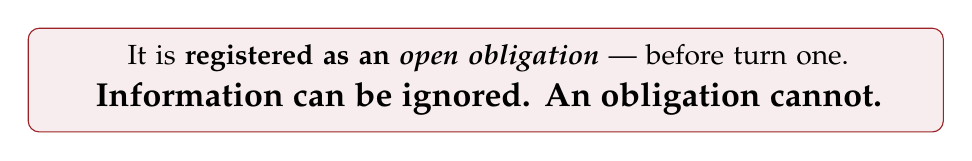
\begin{tikzpicture}
\node[draw, rounded corners, fill=unired!8, draw=unired, text width=11.2cm, align=center, inner sep=6pt]
{It is \textbf{registered as an \emph{open obligation}} --- before turn one.\\[3pt]
\large\textbf{Information can be ignored. An obligation cannot.}};
\end{tikzpicture}
\pause
\medskip
\begin{block}{The division of labour the whole design rests on}
\centering\small
\begin{tabular}{@{}ll@{}}
\toprule
\textbf{deterministic code} & finds the mechanical problems, and makes them \textbf{un-ignorable} \\
\textbf{the model}          & decides what they \textbf{mean} for \emph{this} question \\
\bottomrule
\end{tabular}
\end{block}
\smallskip
\sm{It is not a straitjacket: on the response-rate task the agent looks at the pre-seeded \code{-999}
finding and \textbf{dismisses} it --- correctly, because that column never enters the calculation.
\textbf{We do not force a conclusion. We force the observation to \emph{reach} the decision.}}
\end{frame}

\begin{frame}[fragile]{Ledger 1 --- the Question Contract}
\begin{columns}[T]
\begin{column}{0.53\textwidth}
\textbf{Attacks:} DDB \emph{Constraint} (7.5\%) and the melanoma scope-drop; GBP's ``wrong population /
wrong scale''. \textbf{Failure 2 in Part 1.}
\medskip

\begin{lstlisting}
class QuestionContract(BaseModel):
    estimand:   str   # the exact quantity
    population: str   # WHICH ROWS. the denominator.
    units:      str   # percent? fraction? log?
    constraints: list[str]  # every stated filter
    premises:    list[str]  # what the QUESTION
                            # assumes -- and must
                            # be checked
    question_is_precise: bool   # REQUIRED
    ambiguities: list[str]
\end{lstlisting}
\smallskip
\sm{Pinned into context \textbf{every turn}. Shown to the verifier at submit time.}
\end{column}
\begin{column}{0.47\textwidth}
\begin{alertblock}{Two fields the \emph{evaluation} demanded}
\footnotesize
\textbf{\code{premises}} --- a question can be \emph{wrong}.
\emph{``Which of the \textbf{four} sites had the highest response rate?''} --- there are \textbf{three}.
\emph{``\textbf{Why} do women respond better?''} --- \textbf{they don't}.
\medskip

Without this field the agent answered both, \emph{fluently}, and laundered a false premise into a fact.
\textbf{0/3 $\to$ 3/3.}
\medskip

\textbf{\code{question\_is\_precise}} --- a \emph{required boolean}, and that is the whole trick. With an
optional \code{ambiguities} list the agent left it empty \textbf{every single time}.
\medskip

\centering\textbf{A field the model \emph{may} leave empty is a field the model \emph{will} leave empty.}
\end{alertblock}
\end{column}
\end{columns}
\smallskip
\sm{DDB's melanoma failure \emph{is} question decay. Write the question down as structured state, re-show
it every turn, and \textbf{decay becomes visible} --- to the agent, to the verifier, and to me reading the trace.}
\end{frame}

\begin{frame}[fragile]{Ledger 2 --- the Findings Ledger}
\why{Attacks the notice--act gap directly: GBP's headline, and DDB's 54\% domain-reasoning bucket.}

\begin{columns}[T]
\begin{column}{0.52\textwidth}
Every time the agent notices \emph{anything} --- a sentinel, a wrong dtype, duplicate rows, a group
imbalance --- it must log it:
\begin{lstlisting}
note_finding(
  observation = "biomarker_x has 47 values "
                "of exactly -999.0",
  implication = "missing-data sentinels, not "
                "measurements; they drag the "
                "mean down by ~30%",
  status      = "open",   # open|acted|dismissed
)
\end{lstlisting}
\end{column}
\begin{column}{0.48\textwidth}
\begin{alertblock}{And the rule that makes it bite}
\centering
\code{submit\_answer} is \textbf{hard-blocked} while \emph{any} finding has status \code{open}.
\end{alertblock}
\smallskip
To close one, the agent must either
\begin{itemize}\footnotesize
  \item \gd{act} on it --- pointing at the code step that handled it --- or
  \item \textcolor{unigrey}{\textbf{dismiss}} it --- writing \emph{why} it does not affect the estimand.
\end{itemize}
\smallskip
\sm{Both are recorded. Both reach the final report.}
\end{column}
\end{columns}
\pause
\medskip
\begin{block}{Why this is the right shape for the failure}
GBP's finding is that the model \emph{notices the clue and then treats it as local cleanup.}
This design \textbf{does not let ``local cleanup'' be a terminal state.}
\medskip

And the \code{implication} field is where the \emph{propagation} actually happens --- the agent is forced to
write down \textbf{what this changes} \emph{before} it can proceed. \textbf{That is precisely the step both
papers watch it skip.}
\end{block}
\end{frame}

\begin{frame}{Ledger 2 --- and what it produces}
\begin{block}{The artifact neither paper's system produces}
A run's ledger is a \textbf{complete, auditable record of what the agent noticed and what it did about it.}
\end{block}
\medskip
\centering\scriptsize
\begin{tabular}{@{}p{0.13\textwidth}p{0.38\textwidth}p{0.42\textwidth}@{}}
\toprule
\textbf{status} & \textbf{what it noticed} & \textbf{what it did about it} \\
\midrule
\gd{ACTED} & \code{biomarker\_baseline} has 88 values of exactly \code{-999} & QC-failure sentinel, not a measurement --- excluded before any mean \\
\gd{ACTED} & 48 \code{patient\_id}s appear twice & re-tests; kept the last row per patient \\
\gd{ACTED} & \code{arm} is imbalanced on \code{severity} & \textbf{not randomised} --- stratified, reported the conditional effect \\
\textcolor{unigrey}{\textbf{DISMISSED}} & assay \code{batch B} is on a shifted scale & does not enter a response \emph{rate} --- no effect on this estimand \\
\bottomrule
\end{tabular}
\pause
\medskip
\begin{alertblock}{This is the deliverable --- not the number}
Not \emph{``the model said 0.15''} but \emph{``the model saw the confounding, said what it implied,
adjusted for it, and \textbf{here is the step where it did}.''}
\medskip

\centering One is an \textbf{oracle}. The other is a \textbf{colleague}.
\end{alertblock}
\smallskip
\centering\sm{It costs about 40 lines and one extra tool.}
\end{frame}

\begin{frame}[fragile]{Ledger 3 --- Evidence Grounding}
\why{Attacks DDB's Derivation errors (18.6\%) and Final-answer slips (3.5\%). Failure 4 in Part 1.}

\begin{block}{The rule, stated in the system prompt as an absolute}
\centering\textbf{Every number you report must have been printed by code you ran.}\\
\sm{Estimating is not a permitted operation.}
\end{block}
\medskip
And then it is \textbf{enforced deterministically}, not requested politely:
\begin{itemize}
  \item Regex the numbers out of the answer's \code{evidence} list.
  \item Normalise --- strip commas and percent signs, compare at 4 significant figures, \textbf{also test
        $\times100$ and $\div100$} for the percent-vs-fraction confusion.
  \item Require set containment against the \textbf{concatenated stdout of the whole run}.
\end{itemize}
\medskip
\begin{lstlisting}
REJECTED: the values {0.62} in your evidence never appeared in any executed
output. Compute and print them before citing them.
\end{lstlisting}
\pause
\medskip
\begin{alertblock}{No LLM is involved. It cannot be talked out of it.}
DDB documents this exact failure \emph{in a frontier model}: \emph{``its own code printed the correct
group-level count of 1, but the final tally used the atom-level count of 2.''}
\medskip

An LLM reviewer \emph{might} catch that. \textbf{A regex catches it every time, for free, in fifteen lines.}
\end{alertblock}
\end{frame}

\begin{frame}{The gated exit --- finishing is an \emph{action}, not a default}
\why{DDB: ``The last chance to catch the slip is at the final answer. None of the failing models caught this.''}

\code{submit\_answer} runs four gates \textbf{in order --- cheapest and most deterministic first}:

\medskip
\centering\small
\begin{tabular}{@{}clp{0.52\textwidth}@{}}
\toprule
& \textbf{Gate} & \textbf{Rejects when} \\
\midrule
1 & \textbf{schema}    & pydantic fails $\to$ the \code{ValidationError} text goes back and the model self-repairs \\
2 & \textbf{ledger}    & \emph{any} finding is still \code{open} \\
3 & \textbf{grounding} & a reported number never appeared in real output \\
4 & \textbf{verifier}  & one LLM call --- \textbf{and only if 1--3 passed} \\
\bottomrule
\end{tabular}
\medskip

\centering\sm{\textbf{Never pay for an LLM call to catch what a regex would have caught.}}

\pause
\medskip
\begin{alertblock}{The verifier's critical design detail}
It is a \textbf{different model family} \sm{(self-preference bias --- Zheng et al. 2023)}, and:
\medskip

\centering\textbf{The verifier does not see the agent's reasoning.}
\medskip

\raggedright It sees only the \textbf{Question Contract}, the \textbf{data briefing}, the \textbf{code that ran and what it
printed}, and the \textbf{draft answer}.
\medskip

Show it the chain of thought and it gets \textbf{anchored by the agent's own narrative and rubber-stamps}.
\textbf{The fresh context \emph{is} the mechanism} --- and recall DDB's e3c637: three self-checks, all
agreeing, all on the wrong molecule.
\end{alertblock}
\end{frame}

\begin{frame}{Everything, in one table}
\centering\small
\begin{tabular}{@{}p{0.30\textwidth}p{0.30\textwidth}p{0.33\textwidth}@{}}
\toprule
\textbf{The failure (Part 1)} & \textbf{Where it comes from} & \textbf{What I add} \\
\midrule
It notices and does not act & \rd{GBP notice--act gap};\newline DDB domain reasoning \rd{54\%} & \textbf{Findings Ledger} --- a noticed problem is an \textbf{open obligation}; the exit is blocked until it is discharged \\
\addlinespace
The question degrades & DDB constraint 7.5\%;\newline the melanoma case & \textbf{Question Contract} --- estimand, population, units, premises; \textbf{pinned every turn} \\
\addlinespace
Printed 1, reported 2 & DDB derivation 18.6\%\newline + final-answer slip 3.5\% & \textbf{Evidence Grounding} --- every number must appear verbatim in real stdout. \textbf{A regex.} \\
\addlinespace
Nobody checks at the end & DDB: ``none of the failing models caught this'' & \textbf{Fresh-context verifier} --- different family, \textbf{never sees the reasoning} \\
\addlinespace
\emph{It never noticed at all} & \emph{\rd{neither paper measures this}} & \textbf{The detector} --- deterministic profiler \textbf{pre-seeds the ledger} before turn 1 \\
\bottomrule
\end{tabular}
\pause
\medskip
\begin{alertblock}{Note the last row}
It is the one mechanism \textbf{not} derived from the papers --- it comes from the gap I argued they left
in Section 5.
\medskip

\centering\textbf{It will turn out to be the only one that matters.}
\end{alertblock}
\end{frame}

\begin{frame}{What I deliberately did \emph{not} build}
\why{Restraint is only credible if it comes with a trigger.}

\centering\footnotesize
\begin{tabular}{@{}p{0.17\textwidth}p{0.44\textwidth}p{0.32\textwidth}@{}}
\toprule
\textbf{Not built} & \textbf{Why not} & \textbf{I'd build it when} \\
\midrule
\textbf{Multi-agent}\newline \sm{(planner/coder/critic)} & The state that matters lives in \textbf{one kernel namespace}. Every handoff forces it through the lossy channel of natural language --- \textbf{the exact channel this design works to minimise}. Both papers evaluate \emph{single} agents; DDB gets 51.6\% with one. & The task genuinely decomposes into independent subproblems with narrow interfaces. \sm{(DDB's own future work suggests exactly this.)} \\
\addlinespace
\textbf{A framework}\newline \sm{(LangChain, \ldots)} & It hides \textbf{precisely the parts I am being asked to show judgement on}: context assembly, truncation, error recovery. And with an OpenAI-compatible endpoint there is \textbf{exactly one integration to write}. & Dozens of tool integrations, or a team that needs shared conventions more than transparency. \\
\addlinespace
\textbf{RAG / vector store} & The agent's problem is \textbf{not retrieval}. It is reasoning over a file it \emph{already has}. & Domain knowledge not in the weights and too big for a prompt. \\
\addlinespace
\textbf{A real sandbox} & Out of scope for a prototype --- and \textbf{I say so rather than implying a security claim}. The \code{run\_python} contract is \emph{deliberately identical} to what a container-backed executor would expose, so the swap is \textbf{one class}. & \textbf{Before a single line of untrusted input.} Non-negotiable in production. \\
\addlinespace
\textbf{Fine-tuning} & I have no training data, and \textbf{both papers show the gap is procedural, not knowledge-shaped}. & Once the eval harness has produced a few hundred graded trajectories --- \textbf{then the eval \emph{is} the dataset}. \\
\bottomrule
\end{tabular}
\end{frame}

% ###########################################################################
\section{How would I know it works?}
% ###########################################################################

\begin{frame}{The evaluation \emph{is} the design}
\why{Both supplied papers are, fundamentally, evaluation papers. So I steal their protocol --- and say so.}

\begin{block}{The benchmark}
\textbf{28 tasks, 3 domains.} Ground truth is a \textbf{pandas callable that only the grader ever invokes}
--- it never goes near the agent.
\end{block}
\medskip
\begin{itemize}
  \item \code{penguins.csv} --- real, clean, familiar. The agent should score 100\%, and a guardrail should buy \emph{nothing}.
  \item \code{trial.csv} --- \textbf{synthetic clinical data with a known data-generating process}, built so that plausible-but-wrong analyses give \emph{materially different} answers.
  \item \code{sales.csv} --- \rd{a \textbf{held-out domain}}. E-commerce, not medicine. \textbf{Never designed against.}
\end{itemize}
\pause
\medskip
\begin{alertblock}{Built on GBP's principles, verbatim}
\begin{enumerate}
  \item \textbf{Fully simulated}, so the causal structure is known and nothing can be memorised.
  \item \textbf{Explicit decision points} --- each one mirroring a \emph{documented} failure from Part 1.
  \item \textbf{Ablation-verified numerical separation} --- for every task, \emph{assert} that the naive
        answer and the correct answer differ by \textbf{far more than the grading tolerance}.
\end{enumerate}
\end{alertblock}
\end{frame}

\begin{frame}{The planted decision points}
\centering\footnotesize
\begin{tabular}{@{}p{0.27\textwidth}p{0.22\textwidth}p{0.22\textwidth}p{0.20\textwidth}@{}}
\toprule
\textbf{Trap} & \textbf{The naive path} & \textbf{The correct path} & \textbf{From} \\
\midrule
\code{-999} sentinels in a biomarker column & mean over the raw column & recognise as missing, exclude & GBP notice--act \\
\addlinespace
Re-tested patients appear twice & count rows & deduplicate on \code{patient\_id} & DDB derivation \\
\addlinespace
Assay batch B is on a shifted scale & pool all batches & correct or exclude batch B & GBP ``wrong scale'' \\
\addlinespace
The question restricts to one arm & compute over everyone & \textbf{honour the stated filter} & DDB constraint \\
\addlinespace
\rd{\textbf{Simpson's paradox}} --- treatment looks \emph{worse} overall, \emph{better} in every severity stratum & report the marginal effect & stratify; report the conditional effect & GBP ``wrong population / conceptual level'' \\
\addlinespace
A question whose \textbf{premise is false} & answer it anyway & \textbf{flag the false premise} & DDB melanoma \\
\bottomrule
\end{tabular}
\pause
\medskip
\begin{alertblock}{The Simpson's task is the one I care about}
It is \textbf{the purest possible test of the notice--act gap}: the agent \emph{will} see the imbalance
if it looks, and \textbf{the entire question is whether seeing it changes what it computes.}
\end{alertblock}
\end{frame}

\begin{frame}[fragile]{The separation guard --- and what it caught}
\why{GBP's third principle is the one people skip. It is also the one that saved me.}

\begin{block}{The assertion}
\begin{lstlisting}
assert abs(naive_answer - ground_truth) > 10 * tolerance
\end{lstlisting}
\centering
\emph{For every task:} the plausible-but-wrong path must land \textbf{far outside} the tolerance band.
\end{block}
\medskip
Because if it does not, a lazy analysis \textbf{lands inside the band and is graded \emph{correct}} ---
and \textbf{the benchmark measures nothing at all.}
\pause
\medskip
\begin{alertblock}{I implemented this guard, and it immediately killed two of my own tasks}
\begin{itemize}
  \item A \textbf{median} that turned out to be \textbf{robust to the sentinels I had planted}. \sm{(The trap did nothing.)}
  \item An \textbf{age question} that was \textbf{independent of its own filter}. \sm{(The constraint did nothing.)}
\end{itemize}
\medskip
Both looked \emph{perfectly reasonable}. Both graded \textbf{nothing}.
\medskip

\centering\textbf{The assertion found them. I did not.}
\end{alertblock}
\pause
\smallskip
\centering\sm{\textbf{Write assertions that your benchmark is sound --- not just that the agent passes it.}}
\end{frame}

\begin{frame}{Grading, and what gets measured}
\begin{columns}[T]
\begin{column}{0.46\textwidth}
\begin{block}{Grading --- following GBP}
\textbf{Binary. Programmatic. All-or-nothing.} Pre-specified absolute tolerances.
\medskip

\textbf{No LLM judge for anything a \code{math.isclose} can decide.}
\medskip

\sm{An LLM judge is used \emph{only} for the behavioural tasks no numeric check can grade --- did it flag
the false premise? did it surface the ambiguity? \textbf{5 of 28 tasks}, binary rubric, temperature 0,
different model family.}
\medskip

\sm{\rd{And I did not validate it.} DDB at least validated theirs against other LLMs. I read mine's calls
and they looked right --- which is worth exactly what it sounds like. \textbf{I would rather say so than
let the word ``judge'' imply a rigour I did not buy.}}
\end{block}
\end{column}
\begin{column}{0.54\textwidth}
\begin{block}{What gets measured, per (task, config)}
\begin{itemize}\footnotesize
  \item \textbf{pass rate} --- binary, all-or-nothing.
  \item \rd{\textbf{wrong-attractor rate}} --- \emph{did it land on the \textbf{documented naive} answer?}
  \item \textbf{failure taxonomy} --- every failing run hand-classified into \textbf{DDB's five categories}.
  \item \textbf{process} --- steps, execution errors, errors \emph{recovered from}, tokens, dollars.
  \item \textbf{consistency} --- which tasks are flaky, and are they the ones you would expect?
\end{itemize}
\end{block}
\smallskip
\begin{alertblock}{The metric I am proudest of}
Because every trap has a \textbf{documented} plausible-but-wrong answer with a \emph{numerically distinct}
value, a failure is not just \emph{wrong} --- \textbf{I can tell you \emph{which} wrong}.
\medskip

\textbf{Landing on the naive answer means it fell into the notice--act gap \emph{specifically}.}
\smallskip

\sm{Neither paper reports this. It takes ten lines.}
\end{alertblock}
\end{column}
\end{columns}
\end{frame}

\begin{frame}{The ablations are the actual argument}
\begin{block}{The deal I made with myself, in the design doc, before running anything}
\centering\large
\textbf{If an ablation shows a mechanism does not pay for itself, \emph{it gets cut}.}
\end{block}
\medskip
Each configuration switches off \textbf{exactly one} mechanism:
\medskip

\centering\small
\code{full} \quad \code{no\_briefing} \quad \code{no\_ledger} \quad \code{no\_contract} \quad
\code{no\_grounding} \quad \code{no\_verifier} \quad \code{no\_truncation} \quad \code{no\_guardrails}

\pause
\medskip
\begin{columns}[T]
\begin{column}{0.5\textwidth}
\begin{alertblock}{And: how many runs per cell?}
GBP uses \textbf{10}. DDB uses \textbf{3}.
\medskip

I started at 10, \textbf{like GBP}.
\medskip

\centering\textbf{10 is not enough.}\\
\sm{Section 9 is the story of how I found that out --- \emph{the hard way, and by accident}.}
\end{alertblock}
\end{column}
\begin{column}{0.5\textwidth}
\begin{block}{The check on my own instrument}
Alongside every confidence interval, the number I trust more:
\medskip

\textbf{Run the whole benchmark \emph{twice}. Report the \emph{spread} between the two runs.}
\medskip

\sm{That is not a \emph{model} of the uncertainty. \textbf{It \emph{is} the uncertainty, observed.}}
\end{block}
\end{column}
\end{columns}
\pause
\medskip
\centering
\textbf{If a verdict changes when you run the same experiment again, it was never a verdict.}
\end{frame}

% ###########################################################################
\section{What happened when I ran it}
% ###########################################################################

\begin{frame}{The headline}
\begin{block}{}
\centering
\textbf{4{,}480 runs} $\cdot$ 28 tasks $\cdot$ 3 domains $\cdot$ 8 configurations $\cdot$
\textbf{20 runs per cell} $\cdot$ \textbf{\$16} $\cdot$ \textbf{0 crashes}
\end{block}
\medskip
\begin{columns}[T]
\begin{column}{0.5\textwidth}
\centering\small
\begin{tabular}{@{}lrl@{}}
\toprule
\textbf{Domain} & \textbf{Pass} & \textbf{95\% CI} \\
\midrule
\code{penguins} \sm{clean} & 100\% & [100, 100] \\
\code{trial} \sm{designed against} & 82\% & [62, 97] \\
\rd{\code{sales}} \sm{\textbf{held-out domain}} & \textbf{88\%} & [77, 96] \\
\midrule
\textbf{overall} & \textbf{87\%} & [78, 95] \\
\bottomrule
\end{tabular}
\end{column}
\begin{column}{0.5\textwidth}
\centering\small
\textbf{On the trap tasks --- where a guardrail can bite}
\smallskip

\begin{tabular}{@{}lrr@{}}
\toprule
 & \textbf{pass} & \textbf{fell for the naive answer} \\
\midrule
\textbf{full agent}   & \gd{87\%} & \gd{7\%} \\
\textbf{no guardrails} & \rd{61\%} & \rd{24\%} \\
\bottomrule
\end{tabular}
\smallskip

\textbf{A 3.3$\times$ reduction in the wrong-attractor rate.}
\end{column}
\end{columns}
\pause
\medskip
\begin{block}{And the \emph{shape} matters as much as the size}
On \textbf{clean} data --- lookup, aggregation, groupby, correlation --- \textbf{both configs score 100\%}.
\medskip

\centering\textbf{The guardrails buy nothing where there is nothing to catch}, which is exactly what a
guardrail should do.
\end{block}
\smallskip
\centering\sm{An analysis costs \textbf{\$0.004} and runs in \textbf{11 steps}, on a model at \$0.10/1M tokens.}
\end{frame}

\begin{frame}{The ablation that inverted my own thesis}
\centering\small
\begin{tabular}{@{}lrrlr@{}}
\toprule
\textbf{Remove this} & \textbf{Pass} & \textbf{$\Delta$ vs full} & \textbf{95\% CI} & \textbf{Verdict} \\
\midrule
\emph{(nothing --- the full agent)} & \textbf{87\%} & --- & & \\
\midrule
\rd{the deterministic data briefing} \sm{$\leftarrow$ \textbf{the DETECTOR}} & \rd{60\%} & \rd{$-27\%$} & \rd{$[-40, -15]$} & \rd{\textbf{HURTS}} \\
\emph{every guardrail at once} & 67\% & $-20\%$ & $[-32, -9]$ & \textbf{HURTS} \\
the Findings Ledger \sm{$\leftarrow$ \textbf{my centrepiece}} & 81\% & $-6\%$ & $[-11, -1]$ & \textbf{HURTS} \\
\midrule
the fresh-context verifier & 87\% & $-0\%$ & $[-4, +3]$ & \sm{no detectable effect} \\
observation truncation     & 87\% & $+0\%$ & $[-3, +3]$ & \sm{no detectable effect} \\
the numeric grounding gate & 87\% & $-0\%$ & $[-3, +3]$ & \sm{no detectable effect} \\
the Question Contract      & 88\% & $+1\%$ & $[-2, +5]$ & \sm{no detectable effect} \\
\bottomrule
\end{tabular}
\src{Paired hierarchical bootstrap against the full agent, 10,000 resamples (GBP's scheme)}

\pause
\medskip
\begin{alertblock}{Removing \emph{twenty lines of pandas} hurts more than removing \emph{every gate combined}}
I built this design around \textbf{gates}. The thing carrying it is the \textbf{detector} --- the mechanism
I spent the \emph{least} time on.
\medskip

\centering\Large\textbf{A gate is only as good as the detector feeding it.}
\end{alertblock}
\end{frame}

\begin{frame}{Why --- and it is exactly the gap I accused the papers of leaving}
\begin{block}{The mechanism}
The gates were not \emph{wrong}. They were \textbf{redundant} --- the detector in front of them was already
doing the job. \textbf{Remove the detector and the gates have nothing to gate}, which is precisely why
\code{no\_briefing} (60\%) collapses to roughly the same score as \code{no\_guardrails} (67\%).
\end{block}
\pause
\medskip
\begin{alertblock}{The obvious objection, which I want to raise before you do}
\textbf{GeneBench-Pro says the opposite of what I just said.} They are explicit that \emph{frontier} models
\emph{consistently notice} --- the headroom is in \emph{acting}.
\medskip

\centering\textbf{Because we are not talking about the same model.}
\end{alertblock}
\pause
\medskip
GBP's subjects are \textbf{GPT-5.6-class}. My agent is \textbf{Qwen3-30B-A3B} --- a 30B open model chosen
\emph{precisely because it is weak}.
\medskip
\begin{itemize}
  \item For a \textbf{frontier} model, \code{df.describe()} runs and the sentinel \textbf{is} spotted.
        Noticing is \textbf{the solved half}.
  \item For a \textbf{30B model at \$0.10/1M}, \textbf{noticing is genuinely not reliable} --- and the
        deterministic profiler is \textbf{substituting for a capability the base model does not have}.
\end{itemize}
\end{frame}

\begin{frame}{The boundary condition --- and why it is not a contradiction}
\begin{block}{}
\centering\Large
\textbf{The notice--act gap is a frontier-model problem.}\\[3pt]
\textbf{The \emph{notice} gap is a small-model problem.}
\end{block}
\pause
\medskip
\begin{alertblock}{This \emph{sharpens} GeneBench-Pro rather than challenging it}
Which half of the scaffolding earns its keep depends on \textbf{which half of the job your base model
already does for free}.
\medskip

So \emph{``what should I build on top of the base model?''} \textbf{has no model-independent answer} ---
and GBP's prescription (\emph{``close the gap between noticing and acting''}) is \textbf{right for GPT-5.6
and wrong for almost anything you would deploy on a budget.}
\end{alertblock}
\pause
\medskip
\begin{block}{Which is an argument for owning an \emph{eval harness}, not a list of best practices}
\centering
\textbf{The right answer changes when you change the model --- and only the harness will tell you.}
\end{block}
\pause
\medskip
\centering\sm{\textbf{The falsifiable version is one command away:} re-run this ablation grid on a
frontier model, and the briefing's $-27\%$ should \emph{shrink}. I have not run it. \textbf{If it does not
shrink, I am wrong about the mechanism} --- and I would want to know.}
\end{frame}

\begin{frame}{The instrument lied --- and I only caught it by accident}
\why{I criticised GBP's error bars in Part 1. Then I made the same mistake.}

I ran \textbf{the identical benchmark twice}, either side of a change I had already \textbf{proved was inert}
\sm{(same error rate, same step count, same budget-exhaustion rate --- the prompt differs by one path string)}.

\medskip
\centering\small
\begin{tabular}{@{}lrlc@{}}
\toprule
\textbf{Removing the Findings Ledger} & \textbf{$\Delta$} & \textbf{95\% CI} & \textbf{Verdict} \\
\midrule
\textbf{run A} & \rd{$-11.1\%$} & \rd{$[-18.6, -4.3]$} & \rd{\textbf{``SIGNIFICANT''}} \\
\textbf{run B} & $-1.8\%$ & $[-8.9, +4.6]$ & \emph{``no detectable effect''} \\
\bottomrule
\end{tabular}
\medskip

\raggedright
\textbf{Same code. Same tasks. Opposite conclusions, from 95\% intervals that barely overlap.}
Individual tasks swung \textbf{30--50 points}. One went \textbf{1/10} and then \textbf{6/10}.

\pause
\medskip
\begin{alertblock}{Why it lied --- and it is not a coding bug}
With \textbf{10 runs per cell}, the bootstrap resamples \emph{from the ten outcomes I happened to observe}.
A cell that came back \code{1/10} has a bootstrap distribution centred near 10\% --- and it
\textbf{cannot reach the 60\% the next run produced}.
\medskip

\centering\textbf{A bootstrap gives you the sampling variance of the data you \emph{have}.}\\
\textbf{It knows nothing whatever about the data you did not collect.}
\end{alertblock}
\pause
\smallskip
\centering
\sm{\code{evals/stats.py} opens with a line I wrote myself: \emph{``Confidence intervals, because a point
estimate is how you fool yourself.''} \textbf{And then I fooled myself from \emph{inside} the confidence
interval} --- twice, in opposite directions.}
\end{frame}

\begin{frame}{The error bar I report now}
\centering\small
\begin{tabular}{@{}lrrrrl@{}}
\toprule
\textbf{Remove this} & \textbf{run A} & \textbf{run B} & \textbf{spread} & \textbf{pooled $\Delta$} & \\
\midrule
\textbf{the data briefing} & $-29\%$ & $-25\%$ & \gd{4 pt} & \textbf{$-27\%$} & \gd{\textbf{robust}} \\
every guardrail at once    & $-22\%$ & $-18\%$ & \gd{4 pt} & $-20\%$ & \gd{robust} \\
\textbf{the Findings Ledger} & $-9\%$ & $-3\%$ & \wn{6 pt} & $-6\%$ & \wn{real --- but I will not defend the \emph{size}} \\
the fresh-context verifier & $-1\%$ & $+1\%$ & 3 pt & $-0\%$ & \rd{\textbf{sign flips}} \\
the grounding gate         & $-0\%$ & $-1\%$ & 1 pt & $-0\%$ & \\
the Question Contract      & $-1\%$ & \rd{$+3\%$} & 4 pt & $+1\%$ & \rd{\textbf{sign flips}} \\
\bottomrule
\end{tabular}
\src{Doubled to \textbf{20 runs per cell}. Split the runs in half, compute the ablation on each half, report the spread.}

\pause
\medskip
\begin{alertblock}{Read the spread column, not the point estimate}
The \textbf{briefing} is the only mechanism in this design I would defend \textbf{without hedging}.
\medskip

And the two gates whose \textbf{sign flips} between halves of the same experiment are not weak findings.
\medskip

\centering\Large\textbf{They are not findings. They were weather.}
\end{alertblock}
\pause
\smallskip
\centering\sm{\textbf{The instrument you build to stop yourself believing noise is itself an instrument
--- and it also has to be checked.} Not by reading it. By \textbf{running it twice} and seeing whether it
says the same thing.}
\end{frame}

\begin{frame}{The failure the average hid}
\why{`sales' scores 88\% --- better than the domain I designed against. That was the number I wanted.}

Now read the same runs \textbf{per task}:

\medskip
\centering\small
\begin{tabular}{@{}lrr@{}}
\toprule
 & \textbf{full agent} & \textbf{landed on the \emph{documented naive} answer} \\
\midrule
\code{t4\_simpson} --- Simpson's paradox, \textbf{medical} \sm{(designed against)} & \rd{40\%} & \rd{55\%} \\
\rd{\code{s4\_simpson\_sales}} --- Simpson's paradox, \textbf{held-out domain} & \rd{\textbf{35\%}} & \rd{\textbf{50\%}} \\
\code{b3\_ambiguous} --- \emph{``Did the biomarker improve?''} & \rd{\textbf{5\%}} & --- \\
\midrule
\sm{25 easier tasks, spanning 75--100\%} & \sm{carry the 87\%} & \\
\bottomrule
\end{tabular}

\pause
\medskip
\begin{alertblock}{On the confounded comparison --- the failure both papers were \emph{written about} --- my agent is worse than a coin flip}
And when it fails it lands \emph{exactly} on the confounded answer: it is \textbf{more likely to land on the
naive answer (50--55\%) than on the right one (35--40\%)}.
\end{alertblock}
\pause
\medskip
\begin{block}{}
\centering\Large
\textbf{An aggregate is an average, and an average is where a failure goes to hide.}
\medskip

\raggedright\sm{If you take one methodological point from this talk, take that one --- it is worth more
than any gate in Section 6.}
\end{block}
\end{frame}

\begin{frame}{So what would I build next? Not another gate.}
\begin{block}{First I tried the cheap fix, and it failed}
The one piece of domain knowledge in my system prompt was phrased in \textbf{clinical-trial} language ---
\emph{``if the groups were not \textbf{randomly assigned}, a raw comparison is not a \textbf{treatment
effect}''}. Nothing in an e-commerce table is ``randomly assigned''. Plausible. Testable.
\medskip

I rewrote it in fully domain-neutral terms and re-ran the benchmark. \rd{\textbf{It bought nothing measurable.}}
\end{block}
\pause
\medskip
\begin{alertblock}{Which is a negative result, and the most useful one in the project}
The Findings Ledger works on sentinels and duplicates (\textbf{95--100\%}) because a twenty-line profiler
\textbf{detects} them and hands the agent an obligation it cannot walk past.
\medskip

\centering\textbf{There is no detector for confounding.}
\medskip

\raggedright Nothing computes \emph{``are these groups imbalanced on some third variable?''} So nothing is
seeded, so the gate has nothing to gate, so the agent never notices --- and \textbf{rewording the
instruction does not manufacture an observation}.
\medskip

\centering\textbf{A structural gate can force an observation to \emph{reach} a decision.\\
It cannot \emph{create} an observation that was never made.}
\end{alertblock}
\end{frame}

\begin{frame}{So I built the detector}
\begin{block}{Cross-tabulate every candidate grouping column against every other. Flag the imbalance. Seed it as an obligation.}
\centering
\emph{``\code{arm} is imbalanced on \code{severity}. A raw comparison between arms is not a treatment effect.''}
\medskip

\raggedright\centering\textbf{$\sim$20 lines of deterministic pandas} --- the same twenty lines already worth
$-27\%$ everywhere else in the table.
\end{block}
\medskip
\centering
\code{t4\_simpson}: \gd{\textbf{8/20 $\to$ 13/20}}. \quad The live demo: \rd{$-0.087$} $\to$ \gd{$+0.150$}.
\pause
\medskip
\begin{alertblock}{And then I ran out of API budget before I could re-run the grid with it}
\raggedright So every ablation number in this section describes \textbf{the shipped system \emph{minus} its
newest and, on the evidence, most important component}. \textbf{They are a lower bound.}
\medskip

\centering
I could have shipped the old code so the table matched. \textbf{This seemed better.}
\end{alertblock}
\pause
\begin{block}{The roadmap, then, is not more gates}
\centering\large\textbf{It is more detectors.}
\smallskip

\raggedright\sm{Next: an \textbf{ambiguity} detector --- does the question pin down a population, a measure,
and a direction? Three \code{if}s. \textbf{The detector is the cheapest thing in this design, and it is the
only thing that moves the number.}}
\end{block}
\end{frame}

% ###########################################################################
\section{Limits, and the dashboard}
% ###########################################################################

\begin{frame}{Known limits --- stated plainly}
\why{The papers are scrupulous about theirs, and being caught hiding one is worse than having one.}

\begin{itemize}
  \item \rd{\textbf{The judge is not validated at all.}} 5 of 28 tasks are LLM-graded. DDB at least
        validated theirs against two other judges. I read mine's calls and they looked right --- which is
        worth precisely what it sounds like. \sm{Everything else is \code{math.isclose}.}
  \item \rd{\textbf{The ablation grid cannot separate the ledger from the seeding it feeds.}}
        \code{no\_ledger} removes the blocking gate \emph{and} every pre-seeded finding. The clean
        experiment is \textbf{one extra config and about a dollar}. \textbf{I have not run it}, and I would
        rather point at it than let the ambiguity stand.
  \item \textbf{``4{,}480 runs'' is not 4{,}480 independent trajectories.} The cache key omits the config
        name, so ablations that do not change the prompt \emph{until a gate fires} replay the full agent's
        trajectory. \sm{This is common-random-numbers pairing --- it makes the paired CIs \emph{more}
        precise, not biased --- but the headline count overstates independent work.}
  \item \textbf{The central thesis is a bet, not a result.} \emph{``Scaffolding beats model size''} is why
        this runs on a model 14$\times$ cheaper than the best available. \textbf{I never ran the big model
        with no scaffolding.} One command, \$15. Until then it is a \textbf{design bet with supporting
        evidence}, not a demonstrated fact.
  \item \textbf{I built the traps, so I know them.} The mitigation is the held-out domain --- and the only
        evidence the mitigation works is that \textbf{it caught me twice}.
  \item \textbf{Synthetic data is not the real world.} It is, however, data whose ground truth I can
        \emph{compute} --- which is exactly why GeneBench-Pro simulates too.
\end{itemize}
\end{frame}

\begin{frame}{The dashboard}
\begin{block}{}
\centering\Large
\texttt{http://localhost:8501}
\medskip

\raggedright\centering\normalsize
\code{uv run streamlit run app.py}
\end{block}
\medskip
\begin{columns}[T]
\begin{column}{0.5\textwidth}
\textbf{Tab 1 --- Run the agent}
\begin{itemize}\footnotesize
  \item Ask a question, watch it work.
  \item \textbf{Read the audit trail} --- what it noticed, and what it did about it.
  \item \textbf{Toggle the guardrails off, one at a time, and watch it fail.}
  \item An X-ray of every turn: exactly what went into the model, what came out, how long it took.
\end{itemize}
\end{column}
\begin{column}{0.5\textwidth}
\textbf{Tab 2 --- The evidence}
\begin{itemize}\footnotesize
  \item 4{,}480 runs, 8 ablations.
  \item The per-task table --- \textbf{where the average hides the failure}.
  \item The run where my own confidence interval lied.
\end{itemize}
\end{column}
\end{columns}
\pause
\medskip
\begin{alertblock}{And a caveat I will state before you ask}
The live demo serves \textbf{Qwen3-4B on a GPU I rent} \sm{(vLLM on Modal --- the provider is a
\code{base\_url} and a key, which is exactly why there is no framework here)}. That is
\textbf{7$\times$ smaller} than the model the 4,480-run evaluation was measured on, and the endpoint serves
\emph{one} model --- so the verifier is \textbf{not} cross-family, which my own design argues against.
\medskip

\textbf{Numbers produced live are not comparable to the evaluation.} The dashboard says so itself.
\medskip

\sm{That the 4B \emph{still} lands the Simpson's task (\gd{+0.150}, dodging the \rd{$-0.087$} trap) is a
rather good advertisement for spending the budget on \textbf{scaffolding} rather than on
\textbf{parameters}. It is also $n=1$, so it is an \emph{advertisement}, not a \emph{result}.}
\end{alertblock}
\end{frame}

\begin{frame}{What I would want you to take away}
\begin{enumerate}
  \item \textbf{Both papers agree, from opposite directions, on one diagnosis:} these agents fail by
        \textbf{losing the scientific thread} --- not for lack of knowledge, tools, or compute.
        \sm{Two labs, two domains, two grading philosophies, one conclusion. That convergence is the
        finding.}
  \pause
  \item \textbf{So I spent the entire engineering budget on \emph{procedure}}, not on a bigger model:
        turn the three things that get dropped --- \textbf{the question, the finding, the number} --- into
        state the agent is \textbf{not allowed to drop}.
  \pause
  \item \textbf{And then the evaluation told me I had built the wrong half.} The gates are redundant
        behind a \textbf{20-line detector} I barely thought about.
        \begin{itemize}\footnotesize
          \item[] \gd{\textbf{A gate is only as good as the detector feeding it.}}
        \end{itemize}
  \pause
  \item \textbf{Which is a boundary condition on the papers, not a contradiction of them.} The
        notice--act gap is a \textbf{frontier-model} problem. The \emph{notice} gap is a
        \textbf{small-model} problem. \textbf{Neither paper evaluates a single small model} --- so neither
        could have told me that.
  \pause
  \item \textbf{And the thing I would defend hardest is methodological:} I ran the identical experiment
        twice and it gave me \textbf{two opposite answers}.
        \begin{itemize}\footnotesize
          \item[] \gd{\textbf{The instrument you build to stop yourself believing noise is itself an
                instrument --- and it also has to be checked.}}
        \end{itemize}
\end{enumerate}
\pause
\vfill
\centering
\Large\textbf{Thank you.}\quad\normalsize \texttt{http://localhost:8501}
\end{frame}

% ###########################################################################
\appendix
\section*{Backup}
% ###########################################################################

\begin{frame}{Backup --- per-task results (full agent, $n=20$ each)}
\centering\scriptsize
\begin{columns}[T]
\begin{column}{0.48\textwidth}
\begin{tabular}{@{}llrr@{}}
\toprule
\textbf{Task} & \textbf{Category} & \textbf{Pass} & \textbf{Naive} \\
\midrule
\rd{b3\_ambiguous}        & ambiguous          & \rd{5\%}  & 0\% \\
\rd{s4\_simpson\_sales}   & trap:confounding   & \rd{35\%} & \rd{50\%} \\
\rd{t4\_simpson}          & trap:confounding   & \rd{40\%} & \rd{55\%} \\
b2\_false\_premise\_sex   & false-premise      & 75\%  & 0\% \\
s3\_refunds               & trap:filter        & 75\%  & 0\% \\
t3\_batch\_units          & trap:units         & 85\%  & 10\% \\
s13\_ambiguous            & ambiguous          & 85\%  & 0\% \\
s2\_test\_orders          & trap:outliers      & 85\%  & 0\% \\
s10\_holdout\_rev\_seg    & trap:outliers      & 90\%  & 0\% \\
s11\_holdout\_conv        & trap:constraint    & 90\%  & 0\% \\
s1\_text\_numbers         & trap:dtype         & 90\%  & 10\% \\
s6\_scope                 & trap:constraint    & 95\%  & 0\% \\
s9\_false\_premise        & false-premise      & 95\%  & 0\% \\
h1\_holdout\_mean\_severe & trap:sentinel      & 95\%  & 0\% \\
\bottomrule
\end{tabular}
\end{column}
\begin{column}{0.48\textwidth}
\begin{tabular}{@{}llrr@{}}
\toprule
\textbf{Task} & \textbf{Category} & \textbf{Pass} & \textbf{Naive} \\
\midrule
p1\_lookup                & lookup             & 100\% & 0\% \\
p2\_aggregate             & aggregation        & 100\% & 0\% \\
p3\_groupby               & groupby            & 100\% & 0\% \\
p4\_correlation           & correlation        & 100\% & 0\% \\
s5\_age\_sentinel         & trap:sentinel      & 100\% & 0\% \\
s7\_groupby               & groupby            & 100\% & 0\% \\
s8\_lookup                & lookup             & 100\% & 0\% \\
s12\_holdout\_age         & trap:sentinel      & 100\% & 0\% \\
t1\_sentinel              & trap:sentinel      & 100\% & 0\% \\
t2\_duplicates            & trap:duplicates    & 100\% & 0\% \\
t5\_scope                 & trap:constraint    & 100\% & 0\% \\
b1\_false\_premise\_sites & false-premise      & 100\% & 0\% \\
h2\_holdout\_rate         & trap:duplicates    & 100\% & 0\% \\
h3\_holdout\_scope        & trap:constraint    & 100\% & 0\% \\
\bottomrule
\end{tabular}
\end{column}
\end{columns}
\medskip
\sm{\textbf{Read this table, not the headline.} 25 tasks spanning 75--100\% carry the 87\%. The three
red rows are the ones the papers were written about.}
\end{frame}

\begin{frame}{Backup --- the largest single-task swing, and why it worked}
\begin{block}{\code{t3\_batch\_units} --- assay batch B reporting 10$\times$ too large}
\centering\Large
\rd{\textbf{0/20}} without the guardrails \quad$\longrightarrow$\quad \gd{\textbf{17/20}} with them
\end{block}
\medskip
The machinery works \textbf{exactly as designed}:
\begin{enumerate}
  \item The \textbf{detector} sees the batch on a shifted scale.
  \item It \textbf{seeds the finding} as an \code{open} obligation --- before turn one.
  \item The \textbf{gate} will not let the agent submit until it has been discharged.
\end{enumerate}
\medskip
\begin{alertblock}{The whole thesis of Section 9, in one task}
\centering\textbf{Wherever a detector feeds it, the gate is worth 17 tasks out of 20.}\\
\textbf{Where no detector feeds it (confounding, ambiguity), the gate is worth nothing.}
\end{alertblock}
\end{frame}

\begin{frame}{Backup --- the ambiguity pair, which is more informative than either alone}
\centering\small
\begin{tabular}{@{}llr@{}}
\toprule
\textbf{Task} & \textbf{The question} & \textbf{Pass} \\
\midrule
\code{s13\_ambiguous} & \emph{``Was the campaign successful?''} --- successful by \textbf{which measure}? & \gd{85\%} \\
\code{b3\_ambiguous}  & \emph{``Did the biomarker improve?''} --- and for this assay, \textbf{lower is better} & \rd{5\%} \\
\bottomrule
\end{tabular}
\medskip

\begin{block}{Same mechanism. Opposite outcomes.}
On \code{s13} the gate \textbf{works}: the ambiguity is \textbf{on the surface} (revenue? conversion? per
customer?), the model sees it, declares the question imprecise, and states its reading.
\medskip

On \code{b3} the model fills in \code{question\_is\_precise = True} and \textbf{sincerely believes it}.
Because the thing that makes it imprecise \textbf{is not in the question at all} --- it is in the
\textbf{semantics of the column}. Nothing in the data profile says a \emph{fall} is an improvement.
\end{block}
\pause
\begin{alertblock}{And this one I would not fix in the agent}
That fact is not in the data, not in the column names, not in the question --- and \textbf{not in
\code{data\_dictionary.md} either. I checked.} It exists \textbf{nowhere} in anything the agent is given.
\medskip

\centering\textbf{That is not an agent failure. It is a \emph{documentation} failure.}
\medskip

\raggedright\sm{The correct fix is \textbf{one line in the data dictionary}, not one more gate in the agent.
The reflex in a project like this is to attribute every red cell to the model. \textbf{Some of them are
yours} --- and if your answer to that is a cleverer agent, you have misdiagnosed the bug.}
\end{alertblock}
\end{frame}

\begin{frame}{Backup --- the oddity I will not overclaim}
\begin{block}{Removing \emph{more} made it \emph{better}}
Removing the briefing alone scores \textbf{60\%}. Removing the briefing \textbf{and every gate} scores
\textbf{67\%}. Which is impossible if the gates only ever help.
\end{block}
\medskip
The process metrics show a plausible mechanism:
\medskip

\centering\small
\begin{tabular}{@{}lrr@{}}
\toprule
 & \textbf{steps} & \textbf{findings} \\
\midrule
full agent \sm{(detector + gates)}      & 11.4 & 2.8 \\
\code{no\_briefing} \sm{(gates, no detector)} & 11.0 & 1.5 \\
\code{no\_guardrails} \sm{(neither)}          & 8.7  & 0.4 \\
\bottomrule
\end{tabular}
\medskip

\raggedright
Strip the detector but keep the gates, and the agent \textbf{still has a \code{note\_finding} tool and a
blocked exit --- but nothing informative to put in them.} It logs whatever it stumbles over, spends turns
discharging it, and \textbf{burns budget on ceremony}. Strip the gates too and it simply computes.
\medskip
\begin{alertblock}{\textbf{Gates without a detector may be worse than no gates at all}}
But the paired CI is $[-16.8\%, +5.4\%]$ --- \textbf{it crosses zero}. This is a \textbf{hypothesis with a
mechanism, not a finding}: exactly the kind of story that is \emph{fun to tell} and would be
\emph{dishonest to assert}. It is the first thing I would design an experiment for.
\end{alertblock}
\end{frame}

\begin{frame}{Colophon --- where the numbers come from}
\begin{itemize}
  \item \textbf{Every claim about the papers} was checked against the PDFs by a full re-read. That re-read
        caught \textbf{ten errors in my own earlier write-up} --- four wrong figures and six quotes that had
        drifted from the source \sm{(a spliced quote presented as one sentence; a dropped
        ``with respect to binary labels'' that materially changed a $\kappa$ claim; an oracle denominator
        wrong by 2.5$\times$)}. All are corrected here.
  \item \textbf{Every number about my system} comes from \code{uv run python -m evals.report}, which reads
        \code{evals/results.jsonl} (4,480 runs) --- \textbf{not} from the prose in \code{DESIGN.md}.
        Building the first version of this deck surfaced \textbf{seven stale figures} in that prose. They
        are fixed; the two now agree.
  \item \rd{\textbf{With one exception, where the \emph{script} is the liar.}} \code{report.py} prints a
        headline cost of \textbf{\$3.75}. That is wrong to quote as \emph{spend}: \textbf{77\% of the rows
        are cache replays that record \$0}. On billed runs only, an analysis costs \textbf{\$0.004} and the
        grid cost \textbf{$\sim$\$16}.
\end{itemize}
\medskip
\begin{alertblock}{I nearly ``corrected'' the design doc \emph{down} to \$3.75}
\ldots on the rule \emph{``if the prose and the script disagree, the script is right''}. That rule is right
for every \textbf{rate} in this project and \textbf{wrong for a \emph{sum}} --- because
\textbf{a cache deflates a sum and cannot deflate a proportion}.
\medskip

\centering\textbf{The instrument needs checking too --- and ``trust the script'' is itself an instrument.}
\end{alertblock}
\end{frame}

\end{document}
